\section{Experiments and Results}\label{sec:experimentalresults}
In this section, we present and discuss the experimental results and the validation of the proposed method. Section~\ref{subsec:Database} shows details of the datasets used in the experiments while Section~\ref{subsec:Protocol} describes the experimental protocols employed in this work. Section~\ref{sec:setup} shows the experimental setup of the proposed method regarding its parameters. The experiments in Section~\ref{subsec:analysis} aim at validating our method and choosing its best parameter setup. In addition, Section~\ref{subsec:analysis} addresses important questions regarding the low- and mid-level descriptor extraction procedures: {(1) the best characteristic extracted from Fourier spectrum (e.g., magnitude or phase spectrum); (2) the best measure for spectrum summarization (e.g., energy, entropy, correlation, mutual information, etc);} and (3) the visual codebook size most appropriate for the problem; among others. The remaining subsections compare the proposed method with the best methods reported in the literature including a challenging cross-dataset protocol, whereby we train our method using a dataset and test it with another dataset.

\subsection{Datasets}
\label{subsec:Database}
In this work, we consider four datasets:
%
\begin{itemize}
\item \textbf{Replay-Attack Dataset~\cite{Chingovska:BIOSEG:2012}}: This dataset comprises videos of valid accesses and attacks of $50$ identities. The videos were generated with a webcam with a resolution of $320 \times 240$ pixels and $25$ frames per second (fps). {This dataset contains $200$ valid access videos, $200$ print-based attacks, $400$ mobile-based attacks using an iPhone, and $400$ high-definition attacks using an iPad screen with $1,024 \times 768$ pixel resolution.}

\item \textbf{CASIA Face Anti-Spoofing Dataset~\cite{Zhang:ICB:2012}}: This dataset contains videos of valid accesses and attacks of $50$ identities and considers different types of attacks such as warped photo attacks and cut photo attacks, besides the photos and video attacks. It also considers attacks performed with different image/video quality: 
{(1)~low-quality videos captured by a long-time-used USB camera with $480 \times 640$ pixel resolution; (2) normal-quality videos captured with a new USB camera with $480 \times 640$ pixel resolution; and (3) high-quality videos captured with a Sony NEX-5 camera with $1,920 \times 1,080$ pixel resolution.} In total, it comprises $150$ valid access videos and $450$ video spoofing attacks.

\item \textbf{UVAD Dataset~\cite{Pinto:Unicamp:2013, Pinto:TIFS:2015}\footnote{This dataset is freely available through FigShare \allan{(http://figshare.com/articles/visualrhythm\_antispoofing/1295453)}.}}: This dataset contains valid access and attempted attack videos of {$404$ different people}, all created at Full HD quality, $30$ fps, and nine seconds long. It contains {$16,268$ attempted attack videos and $808$ valid access videos}. {Seven different display devices} were used to simulate the attempted attacks performed upon three acquisition sensors of different manufacturers: {a 9.1 megapixel (MP) Sony CyberShot DSC-HX1, a 10.0-MP Canon PowerShot SX1 IS, a 10.3-MP Nikon Coolpix P100, a 14.0-MP Kodak Z981, a 14.0-MP Olympus SP 800UZ, and a 12.1-MP Panasonic FZ35 digital camera. Figs.~\ref{fig:exemplosVideosValidos} and~\ref{fig:exemplosVideosAtaque} illustrate some examples of this dataset.}
%
\begin{figure*}[!htb]
\centering
\begin{tabular}{c}
	\includegraphics*[width=0.12\textwidth]{facesReais/MAH00938.PNG}
	\includegraphics*[width=0.12\textwidth]{facesReais/MAH01011.PNG}
	\includegraphics*[width=0.12\textwidth]{facesReais/MAH01205.PNG}
	\includegraphics*[width=0.12\textwidth]{facesReais/MAH01241.PNG}
	\includegraphics*[width=0.12\textwidth]{facesReais/MAH01502.PNG}
\end{tabular}
\caption{Examples of valid access video frames for outdoor (first and second images on the left) and indoor (three images on the right) scenes.}
\label{fig:exemplosVideosValidos}
\end{figure*}
%
\begin{figure*}[!htb]
\centering
\begin{tabular}{c}
	\includegraphics*[width=0.12\textwidth]{facesFakes/MAH00938.PNG}
	\includegraphics*[width=0.12\textwidth]{facesFakes/MAH01011.PNG}
	\includegraphics*[width=0.12\textwidth, height=0.082\textheight]{facesFakes/MAH01205.PNG}
	\includegraphics*[width=0.12\textwidth, height=0.082\textheight]{facesFakes/MAH01241.PNG}
	\includegraphics*[width=0.12\textwidth, height=0.082\textheight]{facesFakes/MAH01502.PNG}
\end{tabular}
\caption{Examples of attempted attack video frames for outdoor (first and second images on the left) and indoor (three images on the right) scenes using Sony (first and second columns), Canon (third and fourth columns) and Nikon (last column) cameras.}
\label{fig:exemplosVideosAtaque}
\end{figure*}

\item \textbf{3DMAD Dataset~\cite{Erdogmus:BTAS:2013}}: This dataset comprises valid access and mask attack videos of $17$ different subjects, whose faces were recorded by a Microsoft Kinect sensor. To build a synthetic biometric sample, the authors used frontal and profile face images to make the facial reconstruction. Afterwards, the authors used a 3D printer to build a mask containing facial information of the target person. Spoofing attack simulations were performed by presenting the 3D masks to the same Microsoft Kinect sensor. In total, the authors generated $85$ valid access videos and $85$ attempted attack videos.
\end{itemize}

\subsection{Experimental Protocol}
\label{subsec:Protocol}
We use \redmark{two measures for performance evaluation}: the area under the curve (AUC) and the half total error rate (HTER). \minor{While the former} quantifies the overall ability of a classifier to discriminate between attempted attacks and valid accesses, \minor{the latter} combines the false acceptance rate (FAR) and false rejection rate (FRR) in a specific operating point of the ROC curve into a single measure. HTER is commonly calculated in the operating point in which the FAR is equal to the FRR, known as the Equal Error Rate (EER). \redmark{We use the freely available toolbox Bob~\cite{Anjos:ACMMM:2012} to calculate the AUC and HTER values. Finally,} the employed evaluation protocols follow the ones proposed by the authors of the Replay-Attack, \allan{CASIA,} UVAD and 3DMAD datasets. The source code of all proposed methods are freely available.\footnote{{The source code is freely available for scientific purposes on GitHub \allan{(https://github.com/allansp84/spectralcubes)}, along with this article.}}

\subsubsection{Protocol I} In this experimental protocol, we use the Replay-Attack dataset, which is divided into three subsets: a training set with $300$ attack videos and $60$ valid videos; a development set with $300$ attack videos and $60$ valid access videos; and a test set with $400$ attempted attack videos and $80$ valid access videos. \minor{The training set is used to fit a classification model, the development set to find the EER, whereas the test set is used to report the final error rates.}

\subsubsection{Protocol II} \minor{In this protocol, we use CASIA dataset, divided into two disjoint subsets: training and test sets. \allan{Due to the absence of a development set to estimate a threshold to be applied in the test set and afterwards to calculate the HTER, the official protocol of this dataset recommends to use the training set to build a classifier and then use the test set to report the EER value. To report the results in terms of HTER, the original training set was divided into two subsets, named as training and development sets, in the proportion of $80\%$ and $20\%$, respectively. We use the new training set to find the classification model and the development set to estimate the threshold that gives us the EER, whereas the official test set is used to report the final results in terms of HTER.}
}


%\subsubsection{Protocol II} This is a protocol similar to Protocol I except that we use CASIA dataset instead of Replay-Attack. This dataset is already divided into training and test sets. We split the training into 80\% for actual training and 20\% for development (parameter {optimization}). Finally, the {official} test set was used as the test set.

%\subsubsection{Protocol III} In this protocol, we use the UVAD dataset, which contains one subset with $304$ valid access videos and three subsets, each one with $2,343$ attempted attack videos. Each subset contains attempted attack videos that were generated through spoofing attacks performed in a face biometric system equipped with one of three sensors: Sony, Canon, or Nikon. We use a cross-dataset evaluation protocol here in which we train the classification model with the Replay-Attack dataset and we use UVAD valid access and attempted attack videos to perform the test.

\subsubsection{Protocol III} \minor{In this protocol, we use the UVAD dataset, which contains six subsets comprising valid access and attempted attack videos. Each subset considers attacks against one acquisition sensor: Sony, Kodak, Olympus, Nikon, Canon and Panasonic. Here, we train a classifier using the sensors Sony, Kodak and Olympus, and we test it with videos (valid access and attempted attacks) from three other different manufacturers: Nikon, Canon and Panasonic.}

\subsubsection{Protocol IV} \minor{Here, we use the 3DMAD dataset to evaluate spoofing detection of attacks using 3D masks. The dataset contains $85$ RGB videos that represent valid access and $85$ RGB videos that represent attempted spoofing attacks. As this dataset does not contain explicit subsets, we randomly partitioned the data into three subsets: training, development and testing, and we use Protocol I for testing.}

\subsection{Method Parameterization}\label{subsec:setup}
\label{sec:setup}
For reproducibility purposes, \minor{this section discuss} the parameters whose values are constant in the setup of our method. 

We extract the \redmark{noise signature} from RGB videos using a Gaussian filter with~$\mu = 0$,~$\sigma = 0.5$, and kernel size~$ 3 \times 3$ (Eq.~\ref{eq:ruido}). These values were obtained empirically in~\cite{Pinto:SIBGRAPI:2012}. Next, we extract cuboids of size $32 \times 32 \times 8$ from the Fourier spectrum videos (Eqs.~\ref{eq:mag_spectrum} and~\ref{eq:phase_spectrum}), whose spatio-temporal location is \redmark{chosen randomly based on} a uniform distribution. 

The use of spatial measures produces {low-level $8$-dimensional descriptors} per channel, whereas the use of spatio-temporal measures produces low-level $7$-dimensional descriptors per channel, which gives us a final low-level descriptor of $24$-dimensional and $21$-dimensional, respectively. Finally, the number of cubes extracted from videos is determined by dividing the volume of the video with respect to the cube.

\redmark{Regarding the mid-level descriptors}, the only parameters with constant values are the ones that define the Gaussian kernel used in the soft-assignment coding technique, whose values are~$\mu = 0$ and~$\sigma = 0.04$. Finally, the SVM parameters are found through grid search in  the training data.

\subsection{Experimental Design and Analysis}\label{subsec:analysis}

\begin{table*}
\begin{center}
\begin{footnotesize}
\footnotesize
\caption{{After the statistical analysis, we have found that the factors highlighted with $\dagger$ are the ones that did not present statistical significance when configuring our method, whereas the levels highlighted in bold are the chosen levels.}}
\label{table:DOE}
\begin{tabular}{lp{3.0cm}p{0.70\textwidth}}
\topline
\headcol \textbf{Factor} & \textbf{Levels} & \textbf{Description} \\
\midline
\multirow{1}{*}{LGF} & C, and \textbf{W} & Strategies for extracting the low-level features from video of phase spectrum or video of magnitude spectrum: extraction considering a central region (crop) in each frame (C) and the entire/whole frames (W).\\
\hline
\rowcol \multirow{1}{*}{M} & PE, PH, ME, MH, PMI, MMI, PC, and \textbf{MC} & Characteristics of the frequency spectrum evaluated that can be the phase (P) or magnitude (M) and the measures used for summarizing the spectral information that can be {energy (E), entropy (H), mutual information (MI), or correlation (C)}.\\
\hline
\multirow{1}{*}{CS} & R, and \textbf{K} & Mode of selection of the visual words that compose the visual codebooks: Random (R) or using $k$-means clustering algorithm (K). \\
\hline
\rowcol \multirow{1}{*}{SDD$^{\dagger}$} & S and D & Strategies for generating the visual codebooks: a single visual codebook (S) and class-based visual codebooks (D), one for each data class (spoofing vs non-spoofing). \\
\hline
\multirow{1}{*}{DS$^{\dagger}$} & $80$, $120$, $160$, $200$, $240$, $280$, $320$, and $360$ & Visual codebook sizes. This is an important parameter because the visual codebook size gives us visual codebooks with different degrees of specificities because large visual codebooks can incorporate small clusters of data that appear sometimes in specific cases. \\
\hline
\rowcol \multirow{1}{*}{CP} & hardsum, hardmax and \textbf{softmax} & We evaluate the combination of two strategies in the coding process (hard-assignment and soft-assignment) and two strategies in the pooling process (max-pooling and sum-pooling). \\
\hline
\multirow{1}{*}{C} & \textbf{SVM} and PLS & Classification algorithms. \\
\bottomline
\end{tabular}
\end{footnotesize}
\end{center}
\end{table*}

\redmark{To find the \minor{best method configuration}, we performed} a factorial experiment with replication ($N=3$) followed by an analysis of variance (ANOVA)~\cite{Walpole:PE:2007}. Each experimental unit is represented as a tuple of $n$ objects, each one with a level of a factor. Considering the replications, we have a total of {$9,216$ tuples}, which are used to instantiate the proposed method. The instances of the proposed method are evaluated through the measurement of the value of the system response variable, the AUC value, after running such instances using the Replay-Attack dataset and Protocol~I, using the development set. Next, we collect \redmark{obtained AUC values and then} we performed an ANOVA test to analyze the significance of the effects of the parameters on the \redmark{classification results}. 

With this approach, we can discover which parameters significantly affect the system response variable and also the best configuration of the method~\cite{Hayter:CL:2012}. Henceforth, the \minor{method parameters} are referred to as \emph{factors} and their values as \emph{levels}. Table~\ref{table:DOE} shows a brief description of the factors and their respective levels we consider herein. 

\subsubsection{Low-Level Descriptor Extraction Parameter Analysis (LGF and M)}\label{sec:main_effect_1}

\minor{The low-level feature extraction has two important parameters: the frequency characteristics of the signal (phase or magnitude), and the function used to summarize the information of the temporal cubes extracted from a video. In this work, we evaluate measures that describe spatial information of the temporal cubes (energy an entropy), and measures that describe the temporal behavior of the cubes (mutual information and correlation across time).}

\minor{To find which levels are statistically different for each factor, we perform the Tukey's HSD test (see Fig.~\ref{fig:llf_pvalues}). \redmark{In Figs.~\ref{fig:llf_pvalues}(a)-(b)}, the pairs in comparison whose confidence intervals do not intercept the zero value are statistically different. \allan{Considering the top-5 method configuration obtained in this experiment, we conclude that} the whole frame for extracting features is more interesting than any cropped region in the center of the frame. In addition, the characteristic extracted of the Fourier spectrum and the summarization measure used to generate the low-level feature descriptors \allan{have a great impact} in the method discriminability (Fig.~\ref{fig:llf_pvalues}(b)), \allan{as several comparisons in pairs of features are statistically significant.}}
%
\begin{figure*}[!ht]
\centering
\subfloat[LGF denotes the region of the frame for extracting the low-level features.]{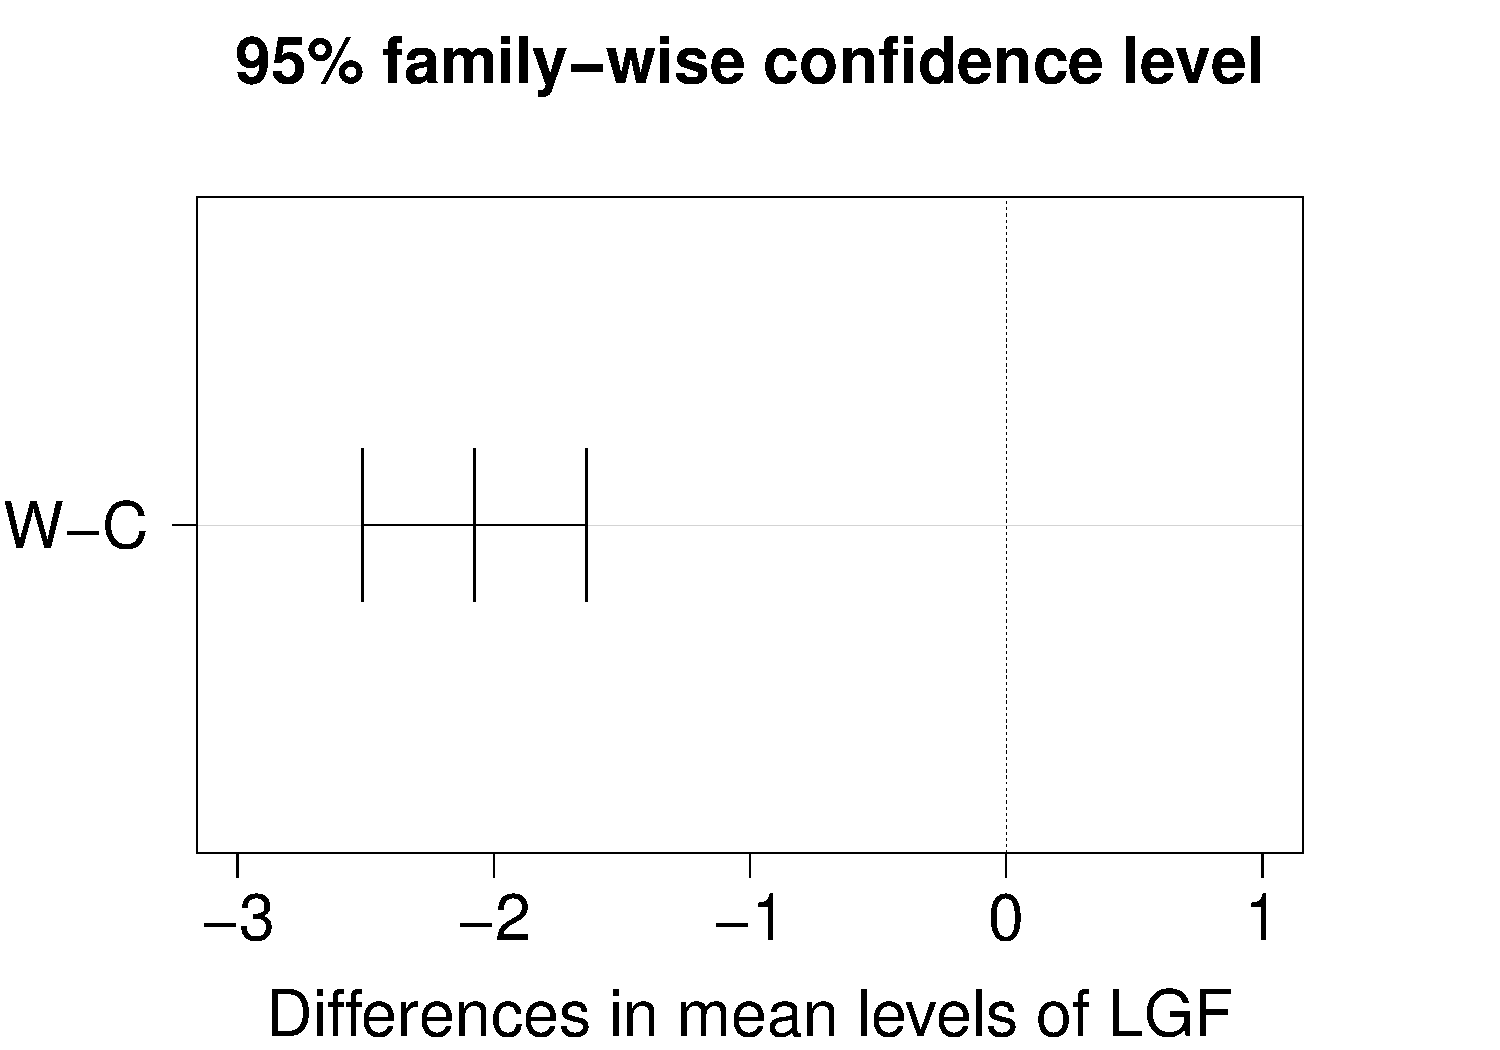
\includegraphics[width=0.21\textwidth]{test_0_auc/LGF}}\hspace{1cm}
\subfloat[M refers to summarization measure and the video of spectra used to generated the low-level descriptors.]{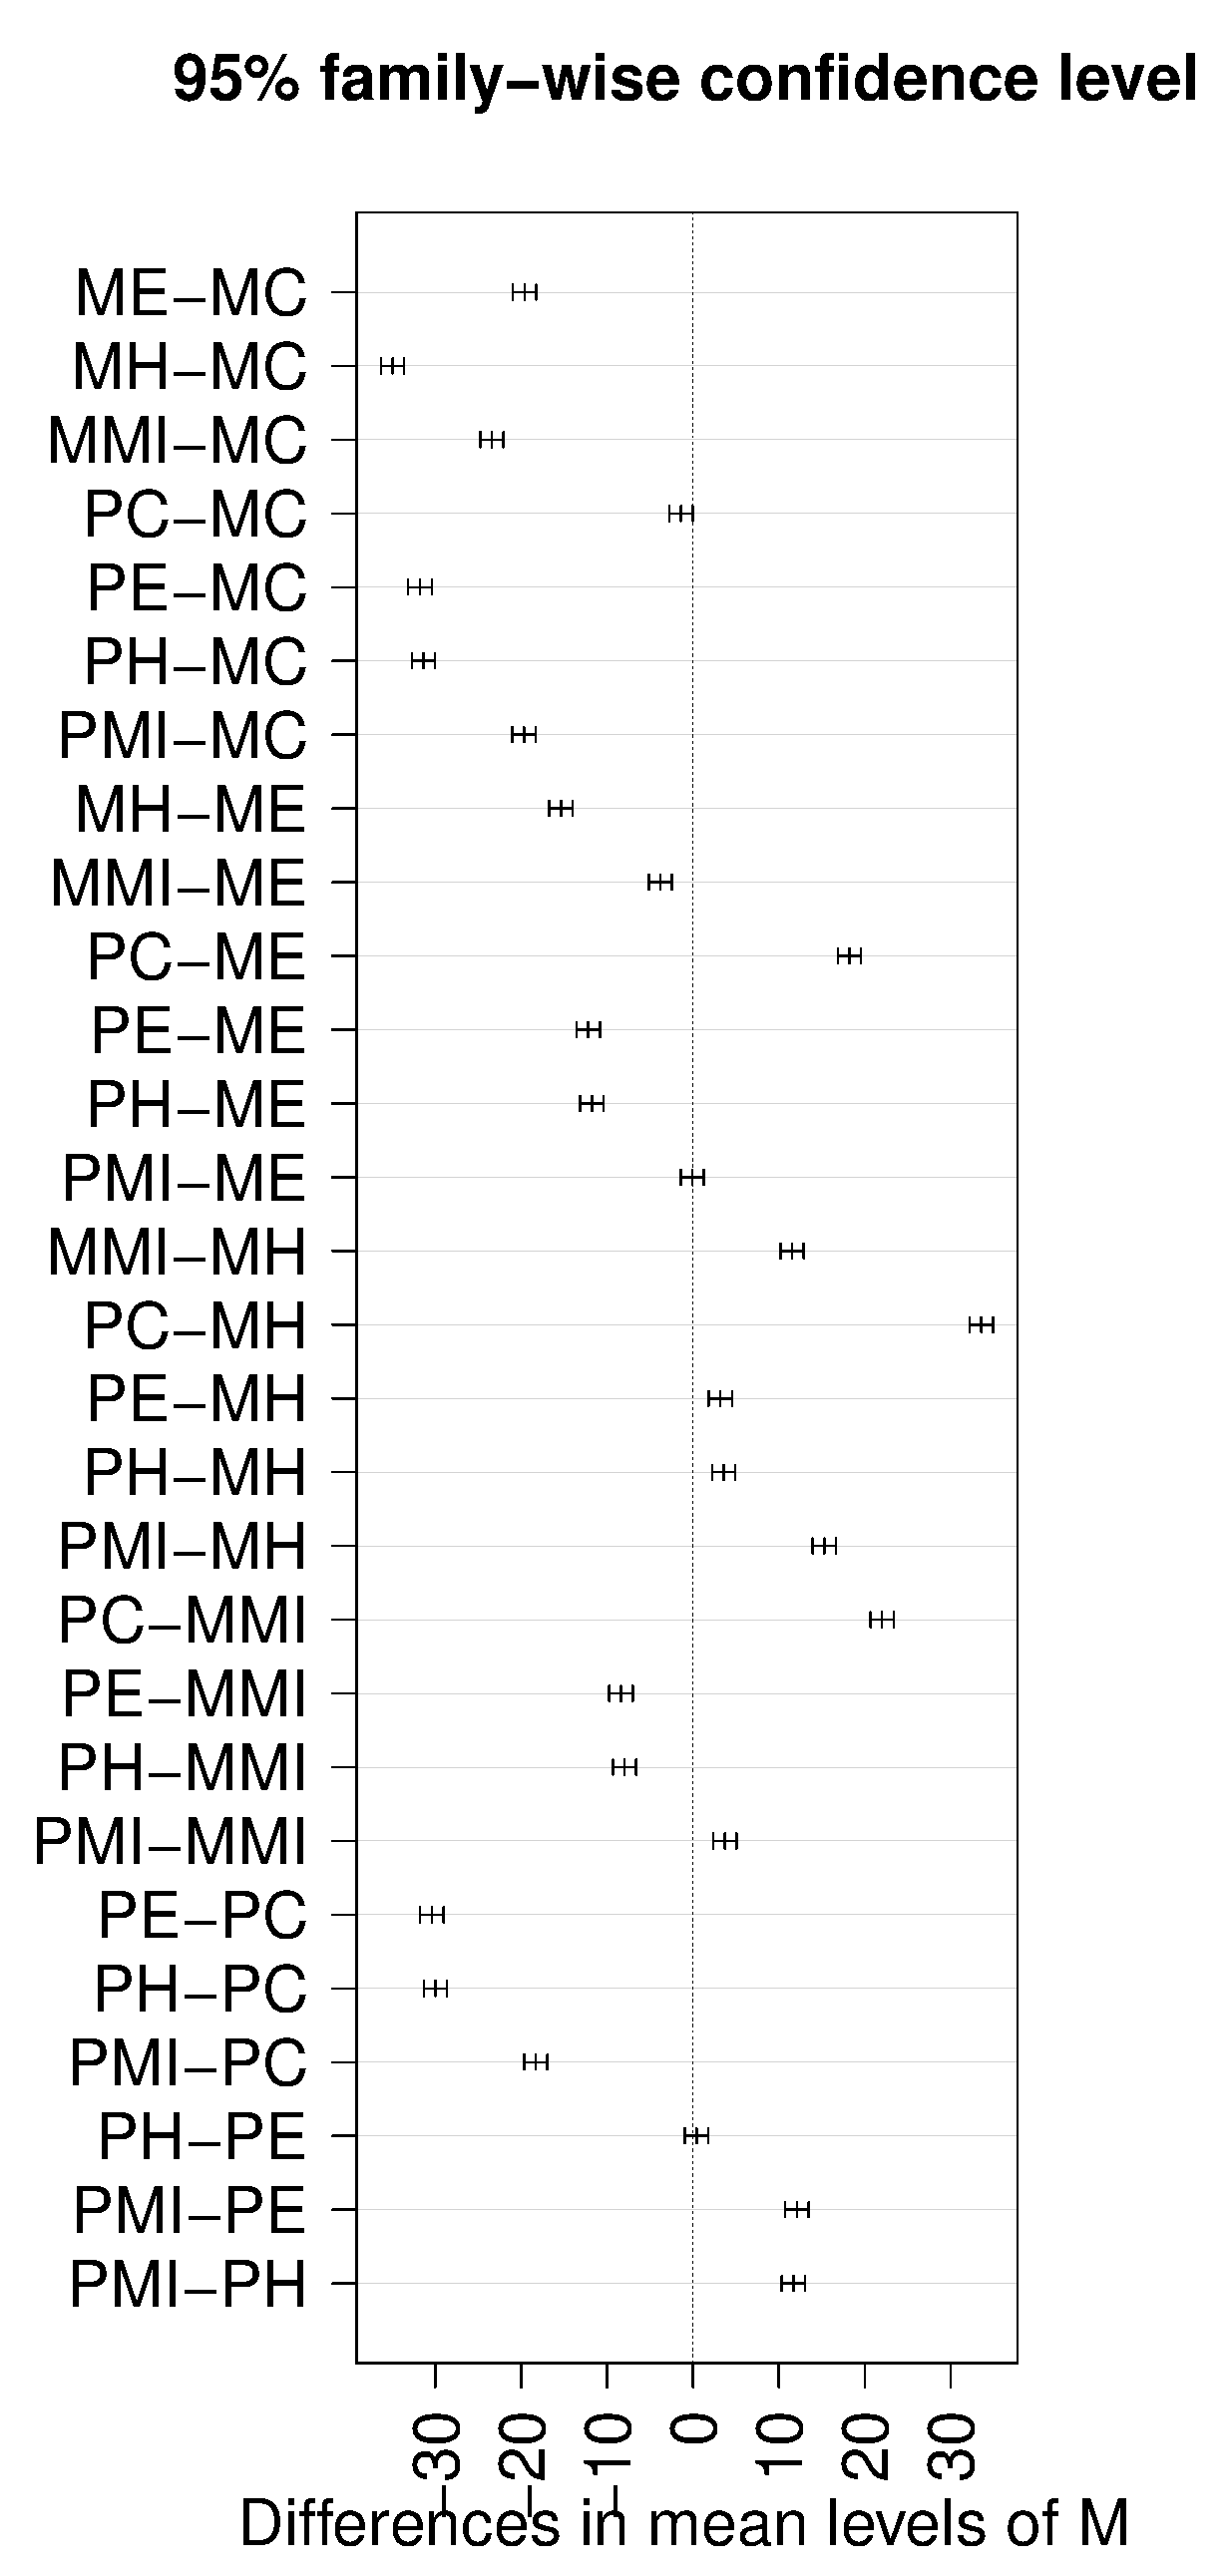
\includegraphics[width=0.35\textwidth]{test_0_auc/M}}\\
\caption{{Confidence interval on the differences between the means of the levels of the factors (a) LGF, and (b) M. For each comparison, the Tukey's HSD test provides an estimation of the differences between mean pairs and their respective confidence intervals, as well the $p$-value for each comparison. All comparisons whose confidence intervals do not contain zero value have a $p$-value lower than $0.05$ and, therefore, are statistically different with a $95\%$ confidence level. (See Table~\ref{table:DOE} to see the description of levels.)\label{fig:llf_pvalues}}}
\end{figure*}

\subsubsection{Mid-Level Descriptor Extraction Parameter Analysis (CS, SDD, DS, and CP)}\label{sec:main_effect_2}
\minor{To construct a discriminative visual codebook, we need to choose the best strategy for selecting the words that compose the visual codebooks (CS) as random or clustering-based,  the visual codebook size (DS), the policy to create the visual codebooks (SDD) as single or class-based, and the pooling and coding strategies (CP).}
%
\begin{figure*}[!ht]
\centering
\subfloat[DS refers to the number of time-spectral visual words present in the visual codebook.]{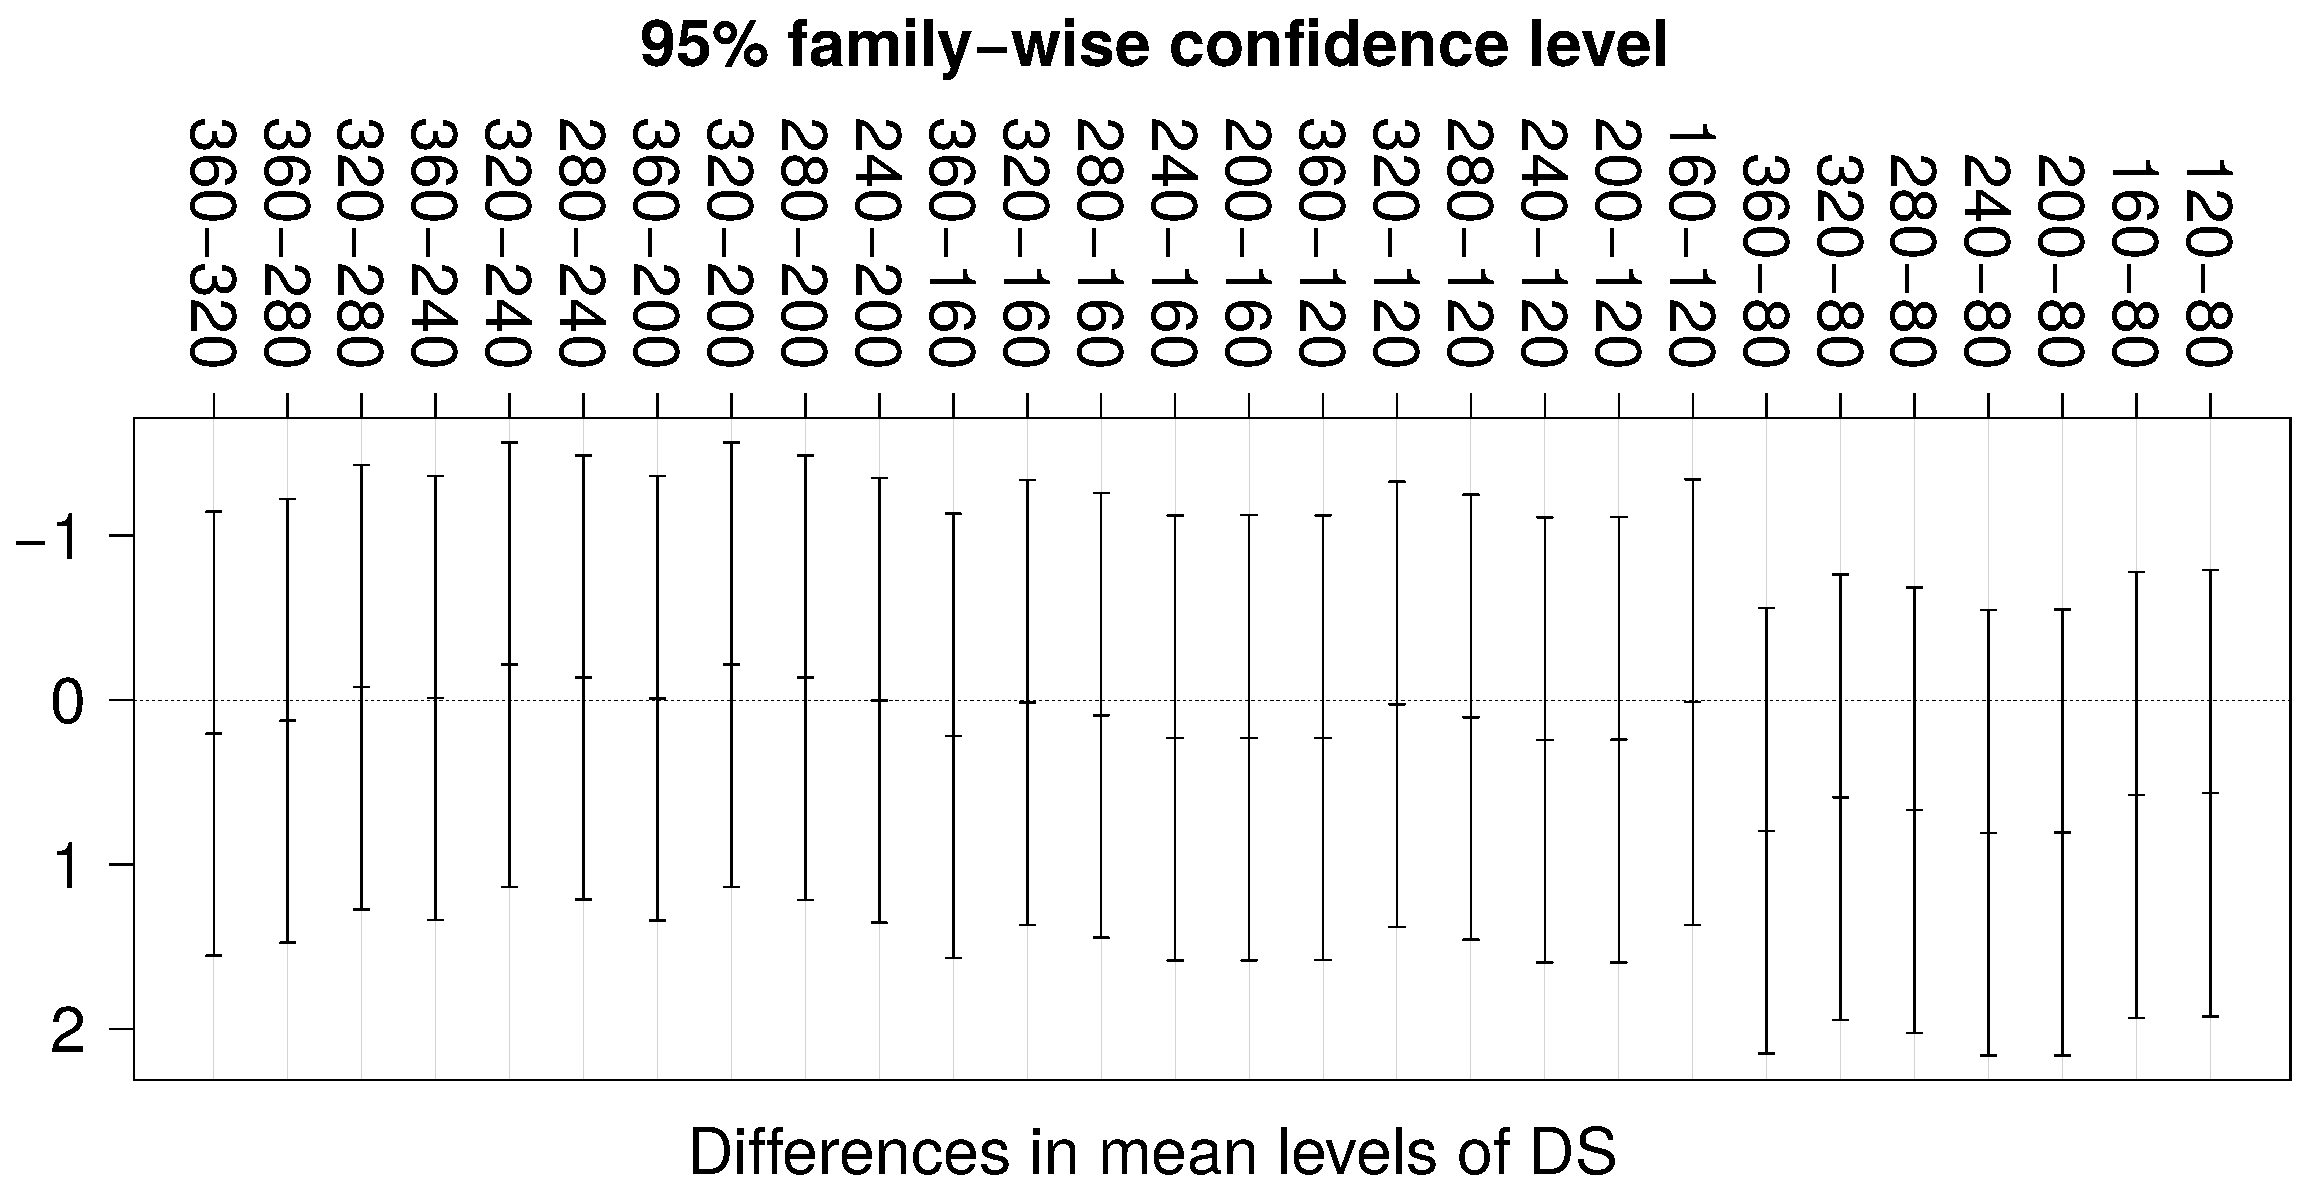
\includegraphics[width=0.3\textwidth]{test_0_auc/DS}} \\
\subfloat[CP denotes the coding and pooling strategies used to build the mid-level descriptors.]{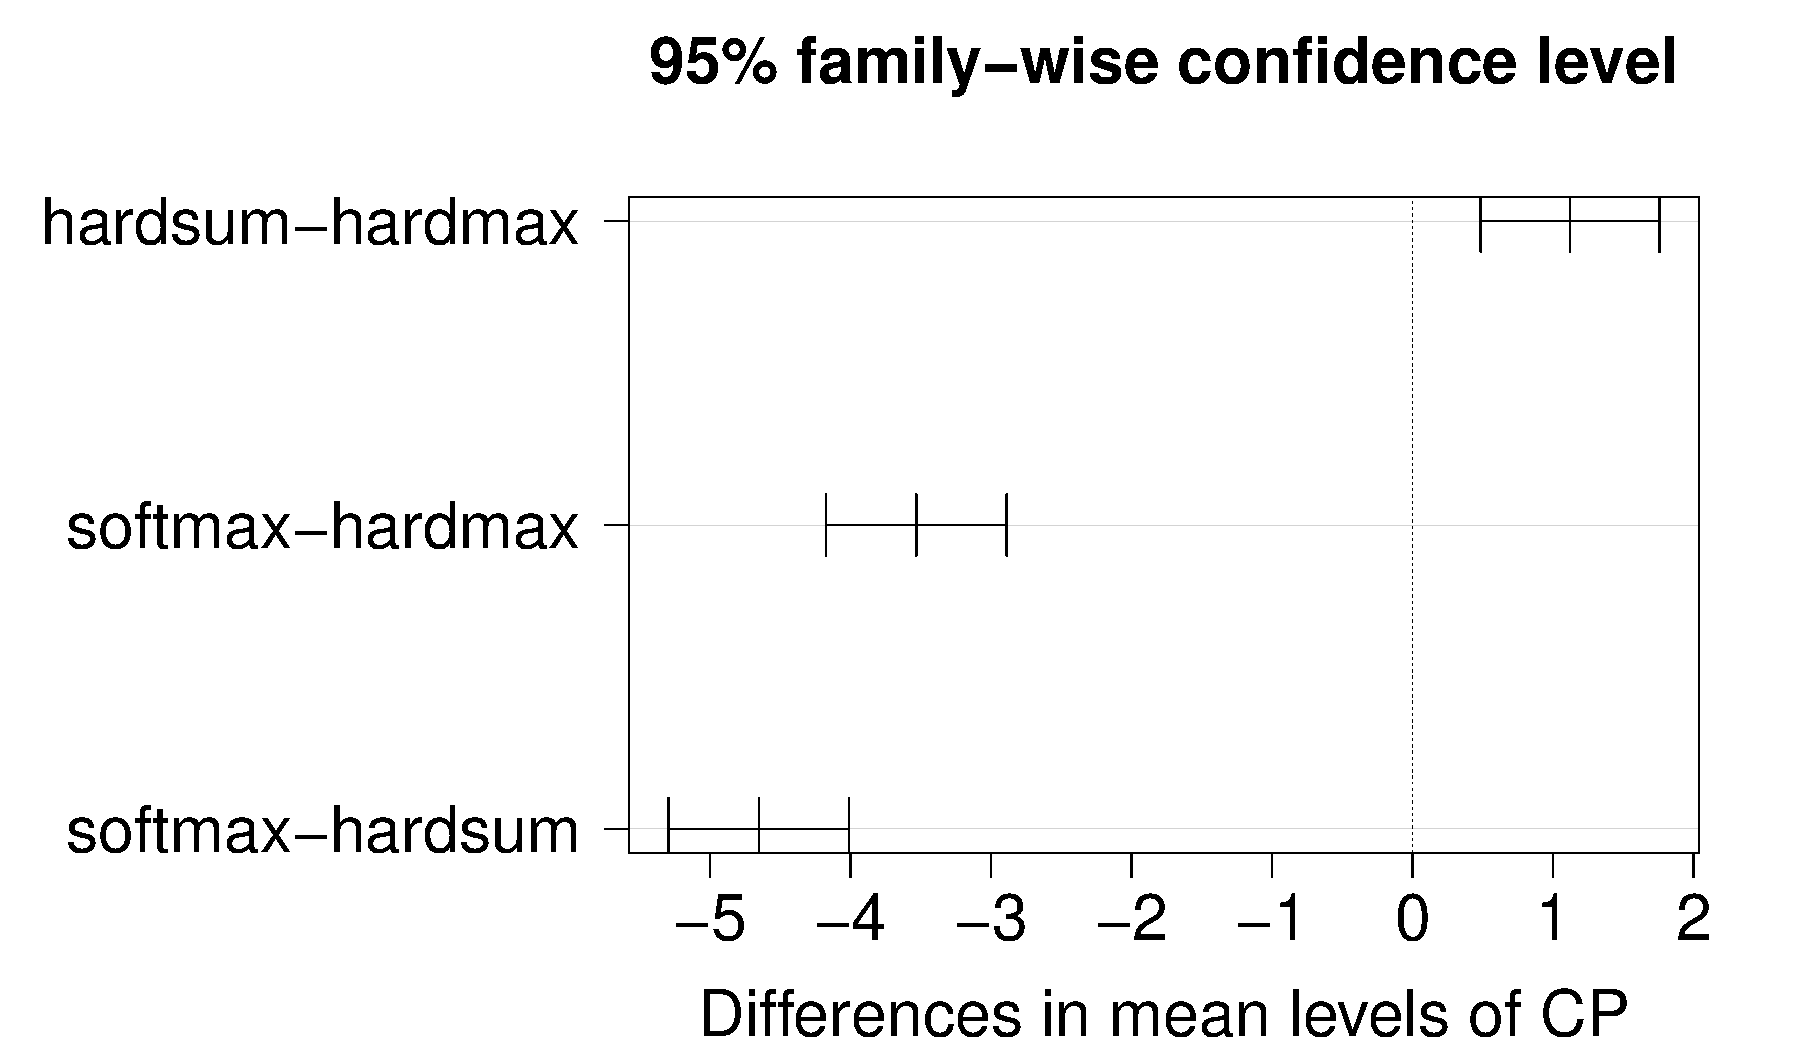
\includegraphics[width=0.25\textwidth]{test_0_auc/CP}}\hspace{5mm}
\subfloat[CS denotes the selection mode of the time-spectral visual words for composing the visual codebook.]{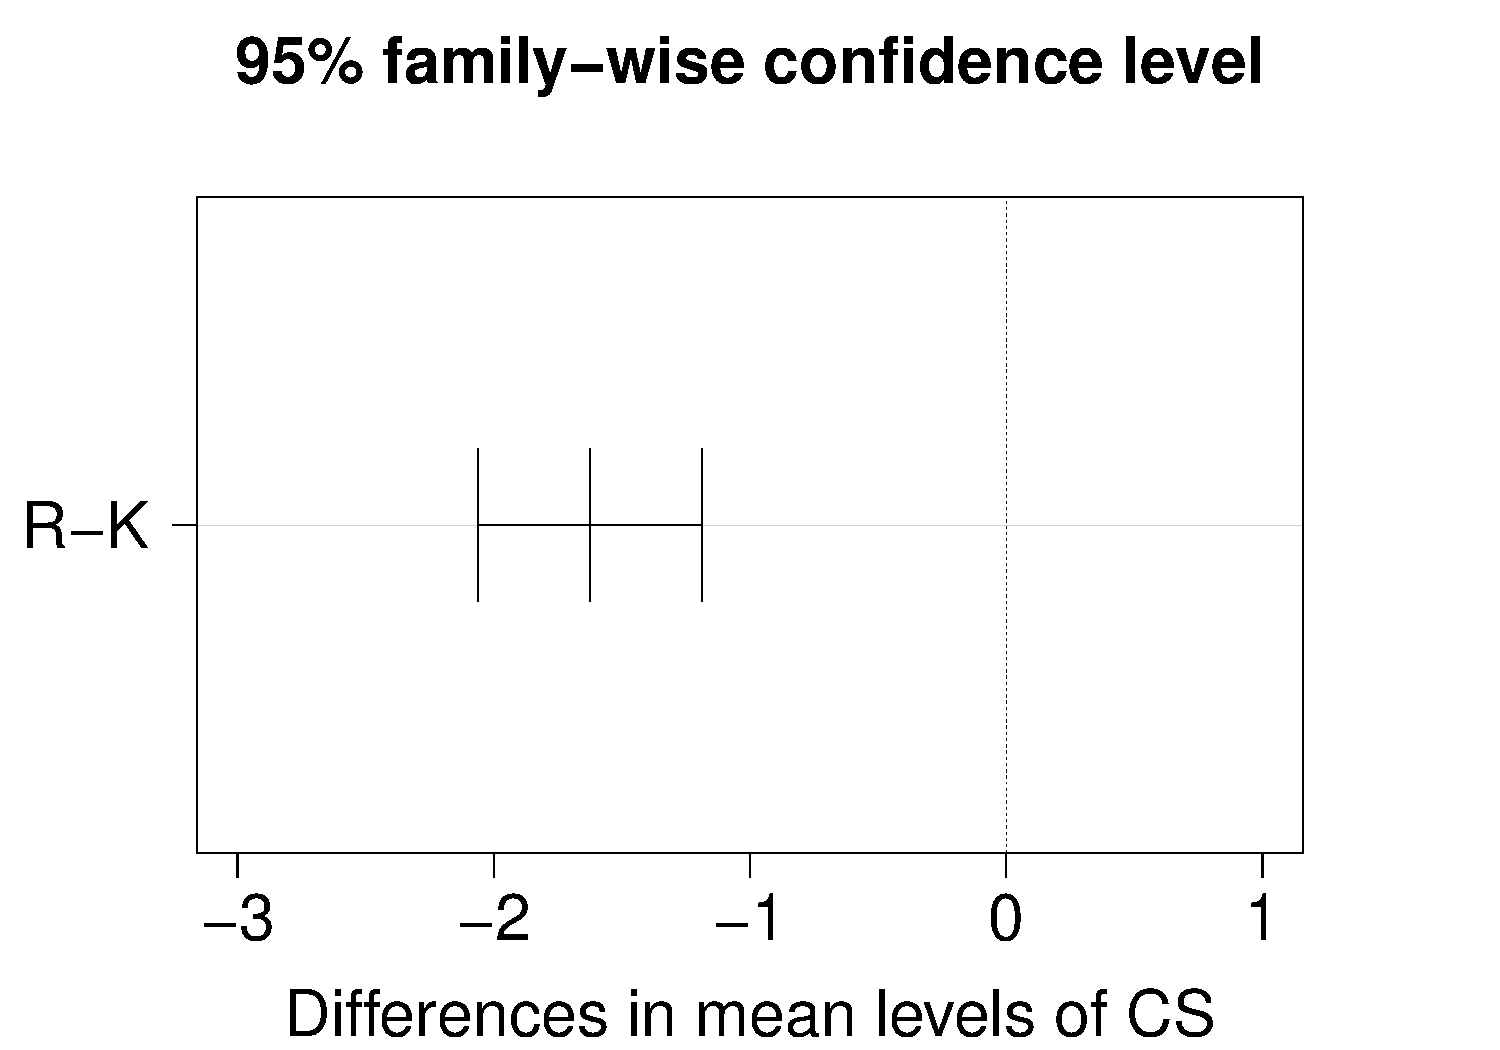
\includegraphics[width=0.22\textwidth]{test_0_auc/CS}}\hspace{2.5mm}
\subfloat[SDD denotes the strategies for generating the visual codebooks, single or class-based visual codebooks.]{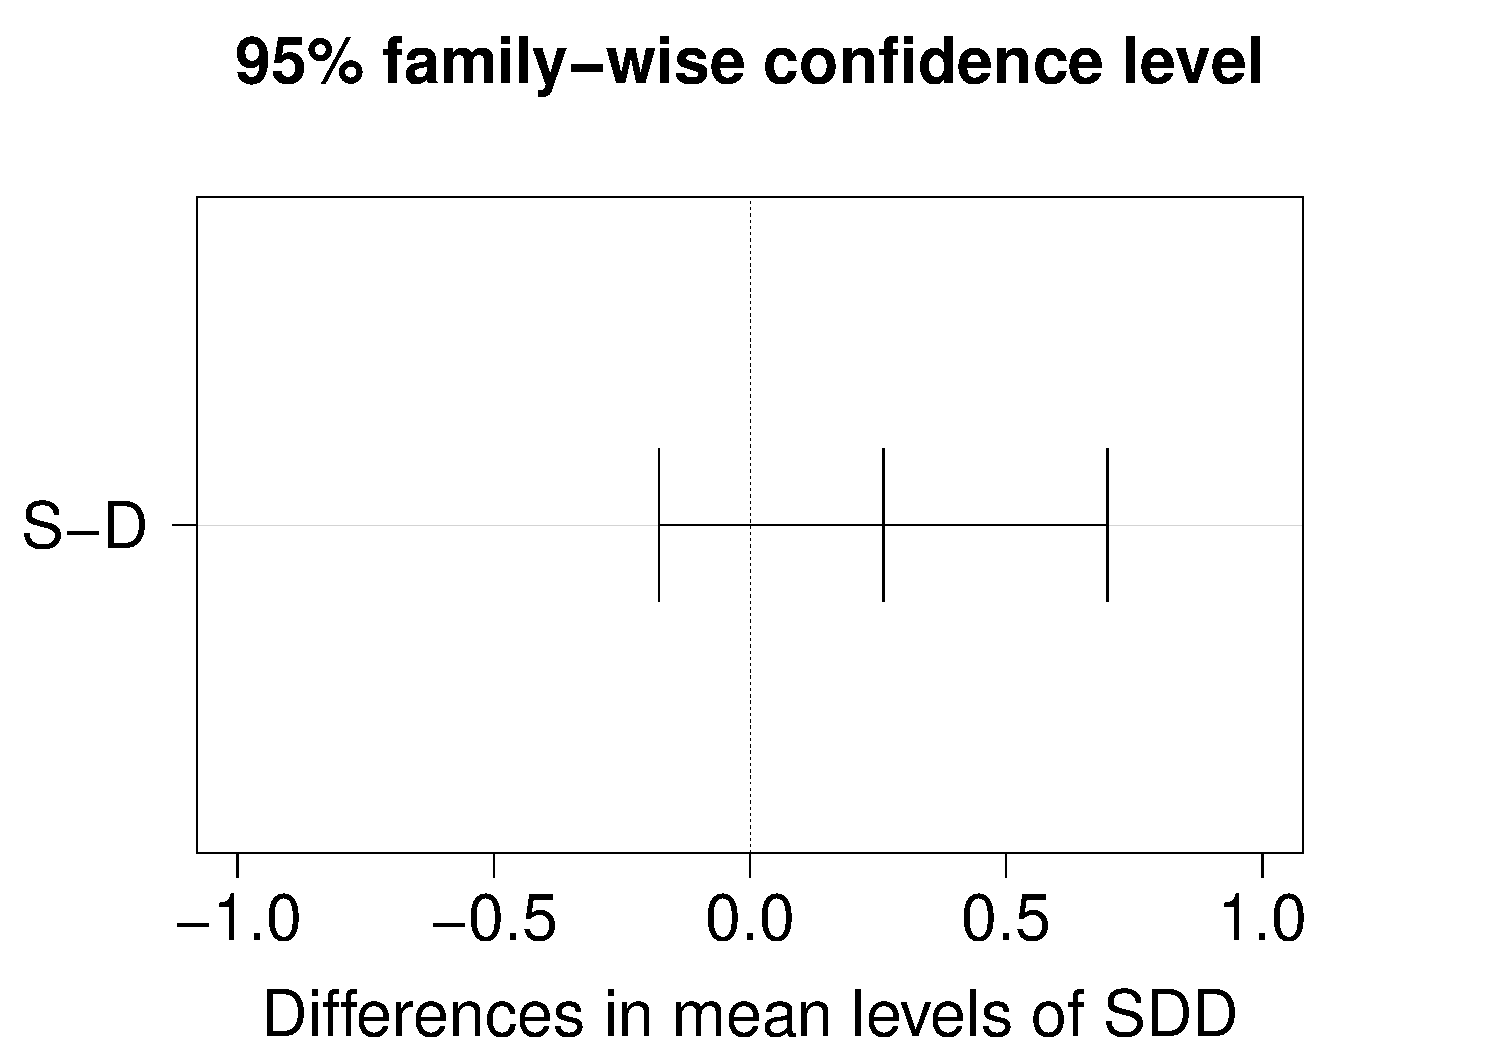
\includegraphics[width=0.2\textwidth]{test_0_auc/SDD}} \\
\caption{Confidence interval of the differences between the means of the levels of the factors (a) DS, (b) CP, (c) CS and (d) SDD. 
All comparisons whose confidence intervals do not contain zero value have a $p$-value lower than $0.05$ and, therefore, are statistically different with a $95\%$ confidence level as it is the case for the comparisons indicated on the (a) $x$ axis and (b-d) $y$ axis. (See Table~\ref{table:DOE} for the description of levels.)}
\label{fig:flf_pvalues}
\end{figure*}

\minor{Fig.~\ref{fig:flf_pvalues} shows the results of the post-hoc test with Tukey's HSD. {In Fig.~\ref{fig:flf_pvalues}(a), we have the results of the statistical analysis for DS parameter (dictionary size), to which was not found statistical significance}. Therefore, we recommend that dictionary size parameter to be optimized according to the application of interest. In turn, Fig.~\ref{fig:flf_pvalues}(b) shows that different pooling and coding processes causes statistically significant impacts on the response variable, and softmax is the recommended choice.}

\minor{In addition, Fig.~\ref{fig:flf_pvalues}(c) shows that the method used to select the words that compose the visual codebook (random vs. clustering-based selection) also presents results that are statistically {significant} with $k$-means being the recommend choice \allan{due to the high performance achieved by models built with visual codebooks generated using $k$-means, during this experiment}. Finally, Fig.~\ref{fig:flf_pvalues}(d) shows that the visual codebook creation strategy (single visual codebook vs. class-based codebooks) does not present statistical difference and, therefore, should also be considered in a future optimization process during the implementation of the method in a real application.}

\subsubsection{Classification Step Parameter Analysis (C)}\label{sec:main_effect_3}
The SVM classifier outperformed PLS classifier with a statistically significant difference  (\textit{$\textit{p}$-value} = $0.00$). We believe that this happened because of the non-linearity of the data as we use a non-linear version of SVM the a linear version of PLS.

\subsubsection{Analysis of Interaction Effects and Choice of the Best Configuration}
\label{sec:best:config}
\minor{After analyzing each factor in isolation, we examine whether there is significant interaction between factors}. In this case, if a small $p$-value is obtained in the interaction effect analysis between two factors, then we can conclude that these factors do not operate independently of each other~\cite{Hayter:CL:2012}. \redmark{Otherwise, there is no evidence of an interaction effect.} 

\minor{First of all, we can see that there is a relationship between the region from which the low-level time-spectral features are extracted (factor LGF) and the spectral information used in the generation of time-spectral descriptors (factor M). When analyzing the magnitude spectrum of the Fourier transform, we see that there is a concentration of low frequency components in the abscissa and ordinate axes. Fig.~\ref{fig:interactions} shows that this interaction between factors LGF and M exists. In addition: (i) we have an increase in the mean of AUC values for measures $MH$, $PH$, $PE$ and $PMI$, when these measures are calculated in the center region of the frames; (ii) we have a decrease in the mean of AUC for measure $PC$; and (iii) we have very small changes in mean values of AUC for $MC$ and $MMI$ when we compare the two strategies for feature extraction.}
%
\begin{figure}[!htb]
\centering
\subfloat[LGF and M interaction. Note that we have a slump in the mean of AUC when setting LGF to W and decrease the number of low-level features.]{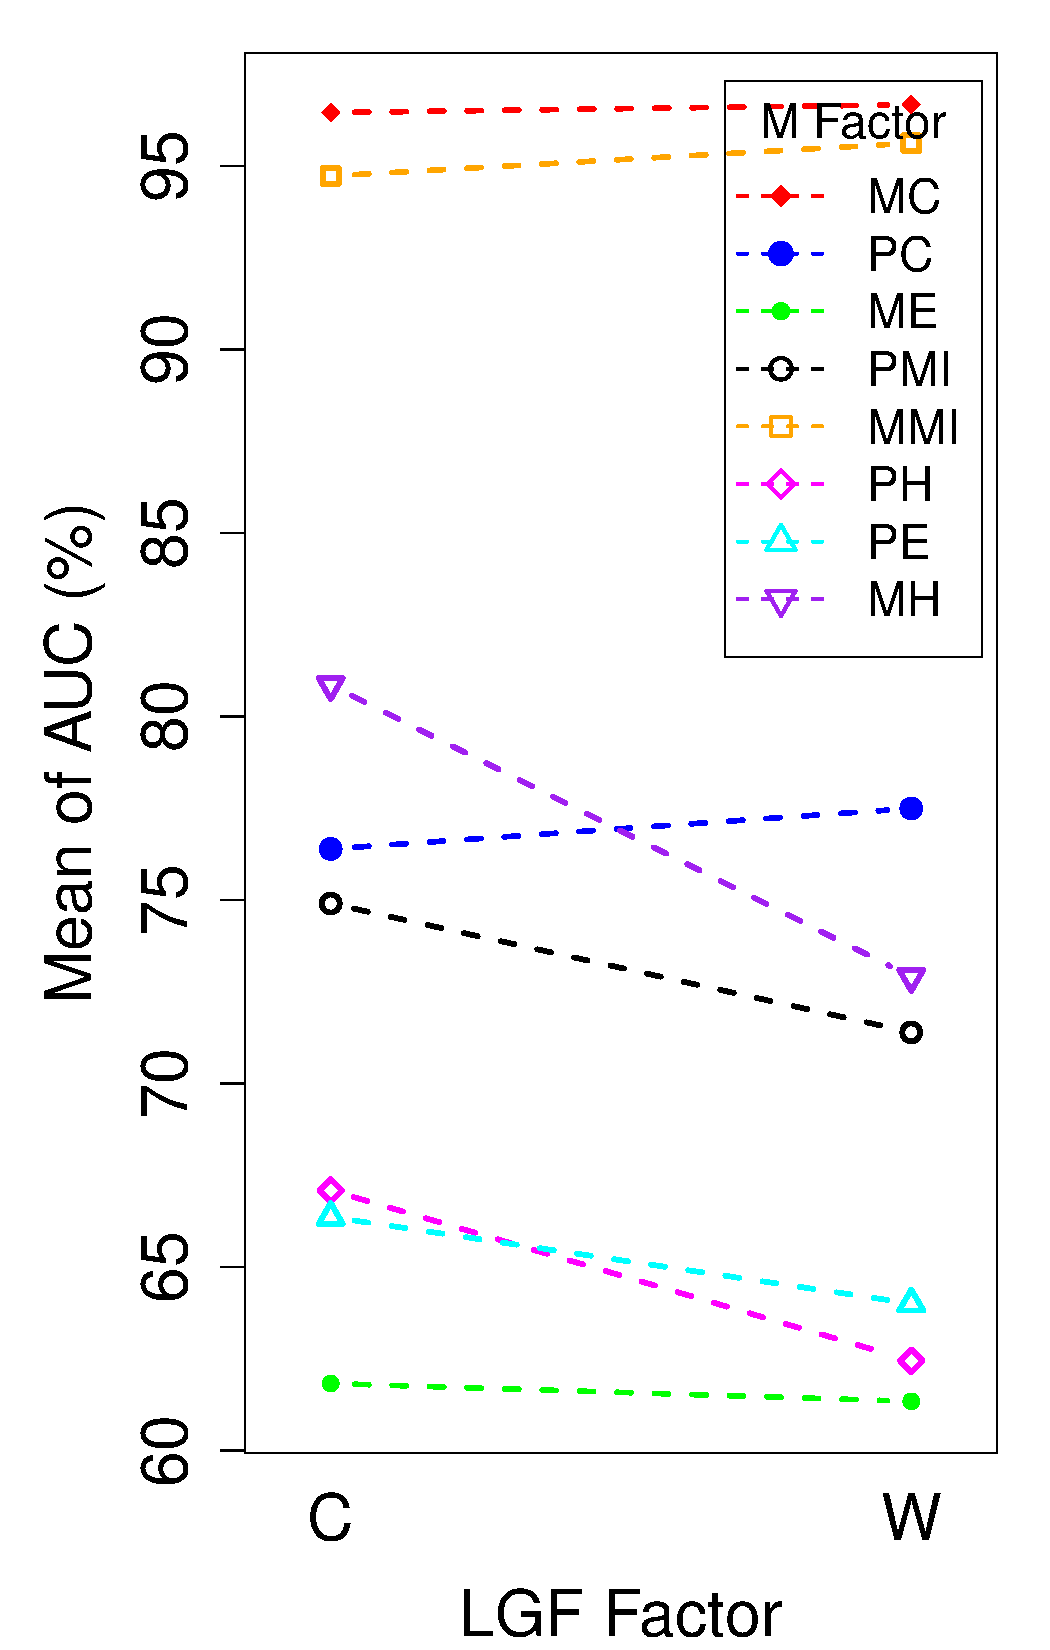
\includegraphics[height=4cm,width=3.5cm]{test_0_auc/LGF_M}}\hspace{0.5mm}
\subfloat[CS and CP interaction. We have a significant increase in the mean of AUC with the hard-assignment when we use $k$-means to select the visual words of the codebooks.]{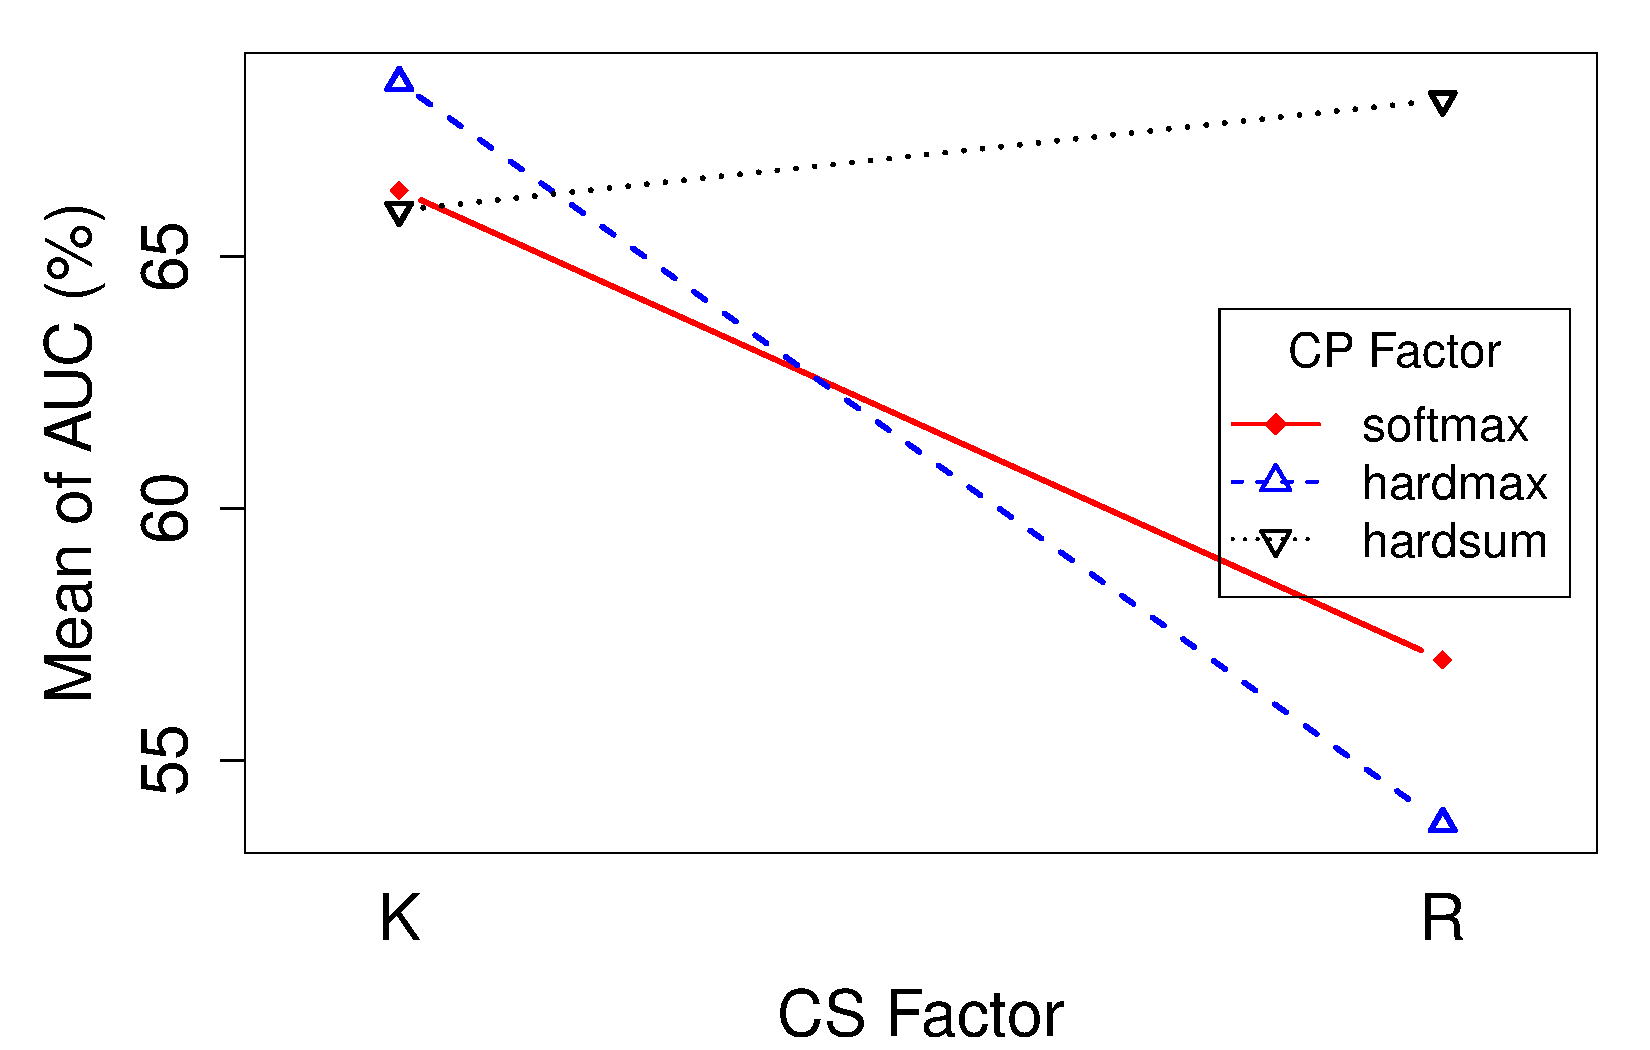
\includegraphics[height=4cm,width=3.5cm]{test_0_auc/CS_CP}}\hspace{0.05mm}
\caption{{Interaction plots between pairs of factors (a) LGF$\times$M and (b) CS$\times$CP. The factor LGF denotes the region in the frame considered for extracting the low-level features, while factor M denotes the statistical measures considered for describing the information of the temporal cubes. Finally, the factor CS denotes the mode of selection of the visual words {from visual codebooks} and the factor CP refers to the strategies used in the coding and pooling process. (See Table~\ref{table:DOE} to see the description of levels.)}}
\label{fig:interactions}
\end{figure}

Finally, the form of selecting the visual words (factor CS) and the method of coding and pooling used in the construction of the dictionaries (factor CP) also presents an interesting interaction. Both factors significantly influence the results, but not in isolation. Fig.~\ref{fig:interactions}(b) shows that the results obtained with hardmax, hardsum and softmax are worse when the visual words are chosen randomly instead of through clustering. 

\subsection{Summary After Analyzing Different Factors and Levels}
{The proposed method presents better results using time-spectral features extracted from magnitude spectrum videos considering the whole frames of a video and using the correlation measure from time-spectral features for generating the time-spectral descriptors.}

{The class-based codebooks \minor{outperform} the single codebook and the selection strategy of the visual words that best fits to the spoofing detection problem is the $k$-means clustering. The most appropriate size for codebooks is $320$ visual words and the softmax outperformed the other coding and pooling strategies. With this configuration, we obtained an AUC of $99.46\%$ and an HTER of $2.75\%$, considering the \allan{test set} of the Replay-Attack dataset~\cite{Chingovska:BIOSEG:2012}. Next, we show experiments and results for this method using this final configuration.}

\subsection{Results}\label{subsec:soa_comparison}
\minor{This section compares the proposed method with others in the literature for the {Replay-Attack~\cite{Chingovska:BIOSEG:2012}, CASIA~\cite{Zhang:ICB:2012} and 3DMAD~\cite{Erdogmus:BIOSIG:2013} datasets. In all experiments, we used the best configuration of the proposed method as discussed in the last section. The parameters that did not present statistical significance (DS and SDD), were fine-tuned for each dataset.}}

\subsubsection{Replay-Attack Dataset}\label{subsec:ra_results}

\minor{We first consider the validation Protocol I~(c.f., Sec.~\ref{subsec:Protocol}) and the Replay-Attack dataset. Table~\ref{table:our_reults} shows the results for the three types of attacks available in this set. Fig.~\ref{fig:det_plot_replay_attack}(a) shows  that attacks performed with high-quality samples are more difficult to detect (HTER of $5.94\%$). This result was expected as high-quality fake samples usually contain less artifacts revealing an attack}.

\minor{In turn, video-based and photo-based attacks were easily detected (HTER of $0.63\%$). Note that video-based spoofing attacks are more susceptible to blurring effects, whereas the photo-based attacks show a large amount of flickering effects due to printing defects. Fig.~\ref{fig:det_plot_replay_attack}(b) shows results obtained considering fixed-support and hand-based attacks, separately. We believe that hand-based attacks are easier to be detected given that small movements of the impostor user during the attack generate more artifacts in the biometric sample causing more disturbances in the \redmark{frequency components.}}
%
\begin{table}[!htb]
\centering
%\linethickness{1.5mm}
\caption{Performance results for the Replay-Attack Dataset.}
\label{table:our_reults}
\begin{tabular}{lcccc}
\topline
\headcol \multicolumn{1}{c}{Dataset} & FAR	& FRR 	& HTER 	& AUC	\\
\midline
High-definition attack 	  & $10.63$ & $1.25$ & $5.94$ & $98.77$ \\
\rowcol Mobile attack 	  & $0.00$  & $1.25$ & $0.63$ & $99.95$  \\
Print attack 			  & $0.00$  & $1.25$ & $0.63$ & $99.86$ \\

\rowcol Hand-based attack & $1.00$  & $1.25$ & $1.13$ & $99.87$  \\
Fixed-support attack 	  & $7.50$  & $1.25$ & $4.38$ & $99.03$ \\

\rowcol \textbf{Overall test set} 
& $\mathbf{4.25}$ &  $\mathbf{1.25}$ &  $\mathbf{2.75}$ & $\mathbf{99.46}$ \\
\bottomlinec
\end{tabular}
\end{table}
%
\begin{figure}
\centering
\subfloat[]{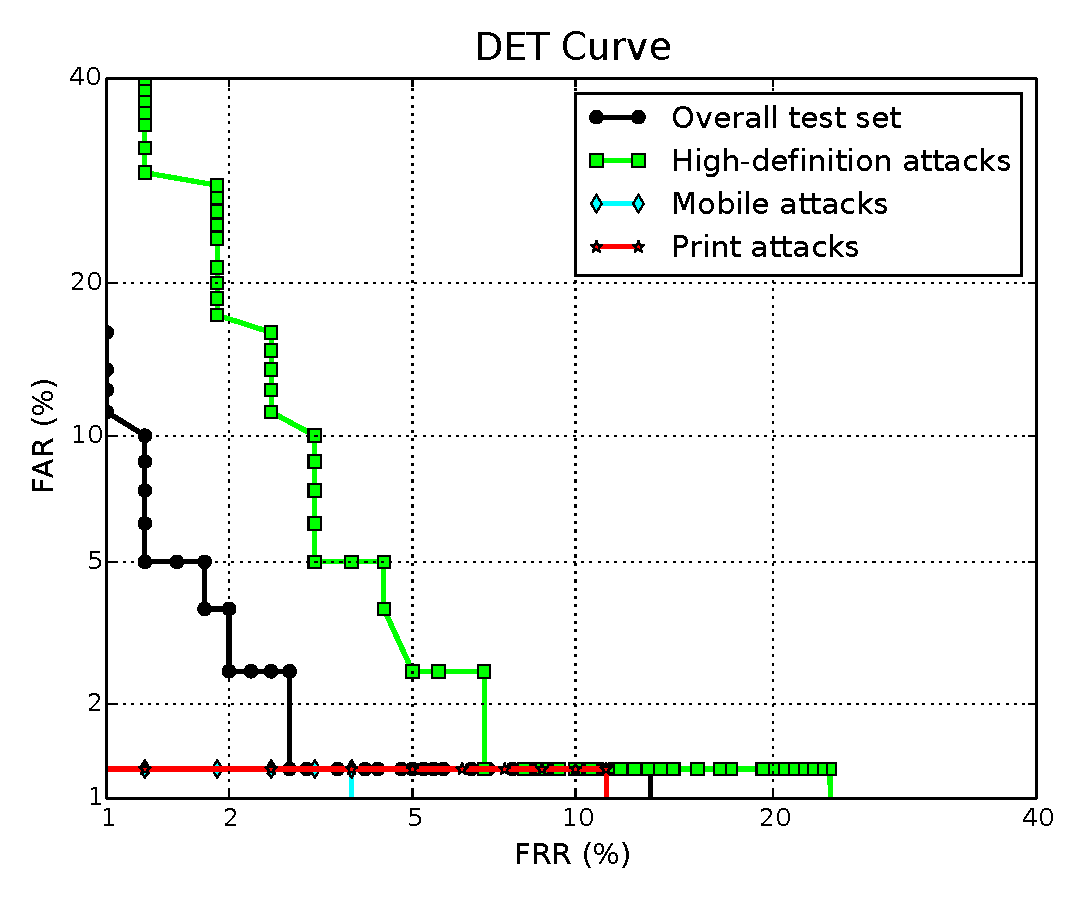
\includegraphics[width=0.45\linewidth]{det_plot_replay_attacks.pdf}}
\subfloat[]{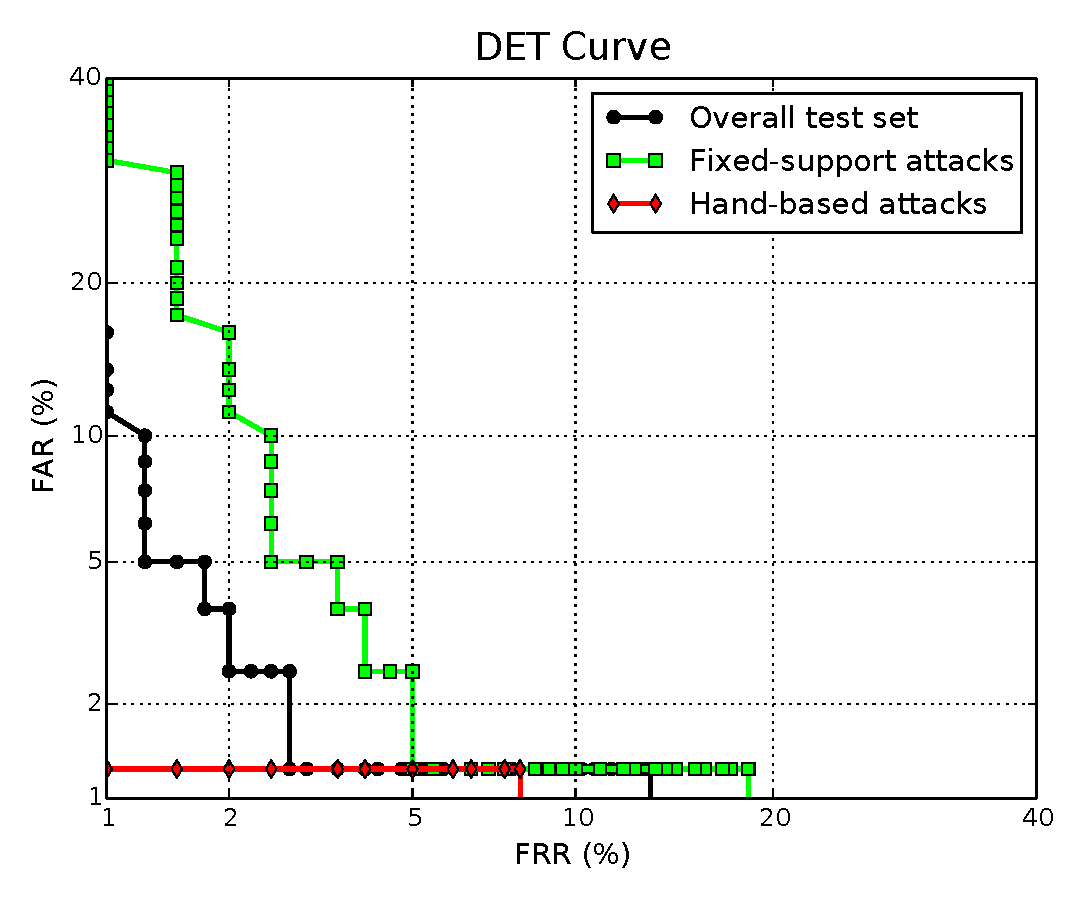
\includegraphics[width=0.45\linewidth]{det_plot_replay_hand_fixed.pdf}}
\caption{{Results obtained on Replay-Attack dataset for each type of attack using fixed-support (a) in contrast with hand-based attacks (b).}}
\label{fig:det_plot_replay_attack}
\end{figure}


\subsubsection{CASIA Face Anti-Spoofing Dataset}\label{subsec:casia_results}
In this experiment, we evaluate the proposed method using the Protocol II (c.f., Sec.~\ref{subsec:Protocol}) and CASIA dataset. 

Table~\ref{table:our_reults_casia} shows the results obtained for the seven {scenarios} of attacks available in this dataset. Fig.~\ref{fig:det_plot_casia}(a) shows that video-based and warp-photo spoofing attacks are easier to be detected by the proposed method (HTER of $ \approx 8\%$). On the other hand, the cut-based spoofing attacks are more difficult to be detected (HTER of $22.22\%$). \redmark{One possible reason for cut-based attacks to be more difficult for detecting is that during an attempted attack based on cut-photos, the photographs are practically in the same position during all the time, generating fewer artifacts along time, whereas for the attempted attacks based on warped-photos, the photographs are bent during the attack to simulate facial motion. In addition, we believe that video-based attacks were easier to be detected because of the inevitable downsize of the high-resolution samples by the screen device used during attack, as also reported by CASIA's authors~\cite{Zhang:ICB:2012}. In this case, many evidences of attempted attacks are generated and added to the fake sample.} 

As for the quality of the acquisition (Fig.~\ref{fig:det_plot_casia}(b)), the proposed method showed better results for attacks carried out with low-quality videos. An interesting result is the best performance of the method to deal with high-resolution videos than normal quality videos. \redmark{We believe that any conclusion would be precipitous because many factors can influence the noise level of a sensor such as sensor imperfections (e.g., appearance of hot pixels, dead pixels, as well as pixel traps under different acquisition conditions). Several works in the literature have explored these issues. For instance, thermal action has a considerable impact over pattern noise of a digital camera and appearance of defective pixels~\cite{Chen2007,Lukas:TIFS:2006,Rocha:2011:VUC}. As we do not assure that the captures/recaptures happened under similar acquisition conditions, it is wiser only to point out the existence of classification differences in this case.}
%
\begin{table}[!htb]
\centering
%\linethickness{1.5mm}
\caption{Performance results for the CASIA dataset.}
\label{table:our_reults_casia}
\begin{tabular}{lcccc}
\topline
\headcol \multicolumn{1}{c}{Dataset} & FAR	& FRR 	& HTER 	& AUC	\\
\midline
		Low quality		  & $10.00$ & $10.00$ & $10.00$ & $98.11$ \\
\rowcol Normal quality    & $17.78$ & $20.00$ & $18.89$ & $87.67$ \\
		High quality 	  & $13.33$ & $13.33$ & $13.33$ & $95.04$ \\
\rowcol Warp photo attack & $7.78$  &  $8.89$ &  $8.33$ & $96.05$ \\
		Cut photo attack  & $22.22$ & $22.22$ & $22.22$ & $87.27$ \\
\rowcol Video attack 	  &  $8.89$ &  $8.89$ &  $8.89$ & $96.41$ \\
\textbf{Overall Attack}   & $\mathbf{14.07}$ &  $\mathbf{14.44}$ &  $\mathbf{14.26}$ & $\mathbf{93.25}$ \\
\bottomline
\end{tabular}
\end{table}
%
\begin{figure}
\centering
\subfloat[]{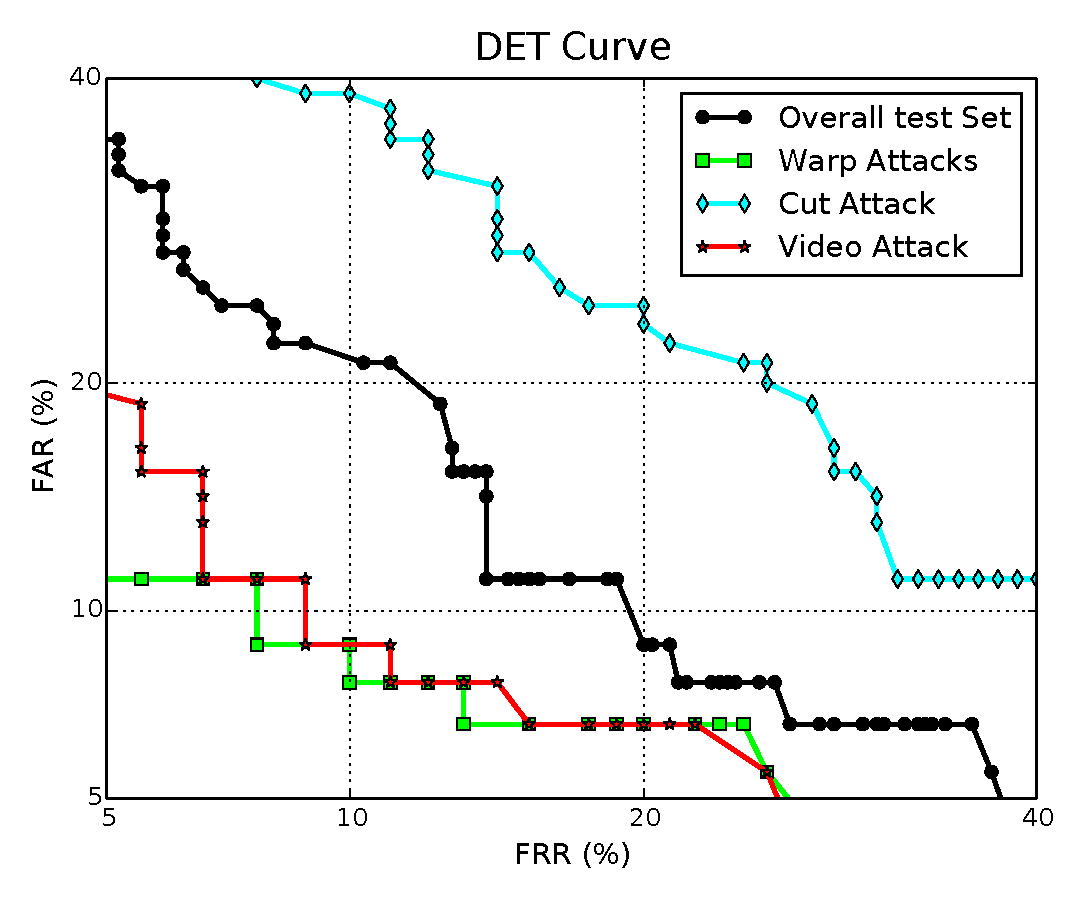
\includegraphics[width=0.45\linewidth]{det_plot_casia_type_attacks.pdf}}
\subfloat[]{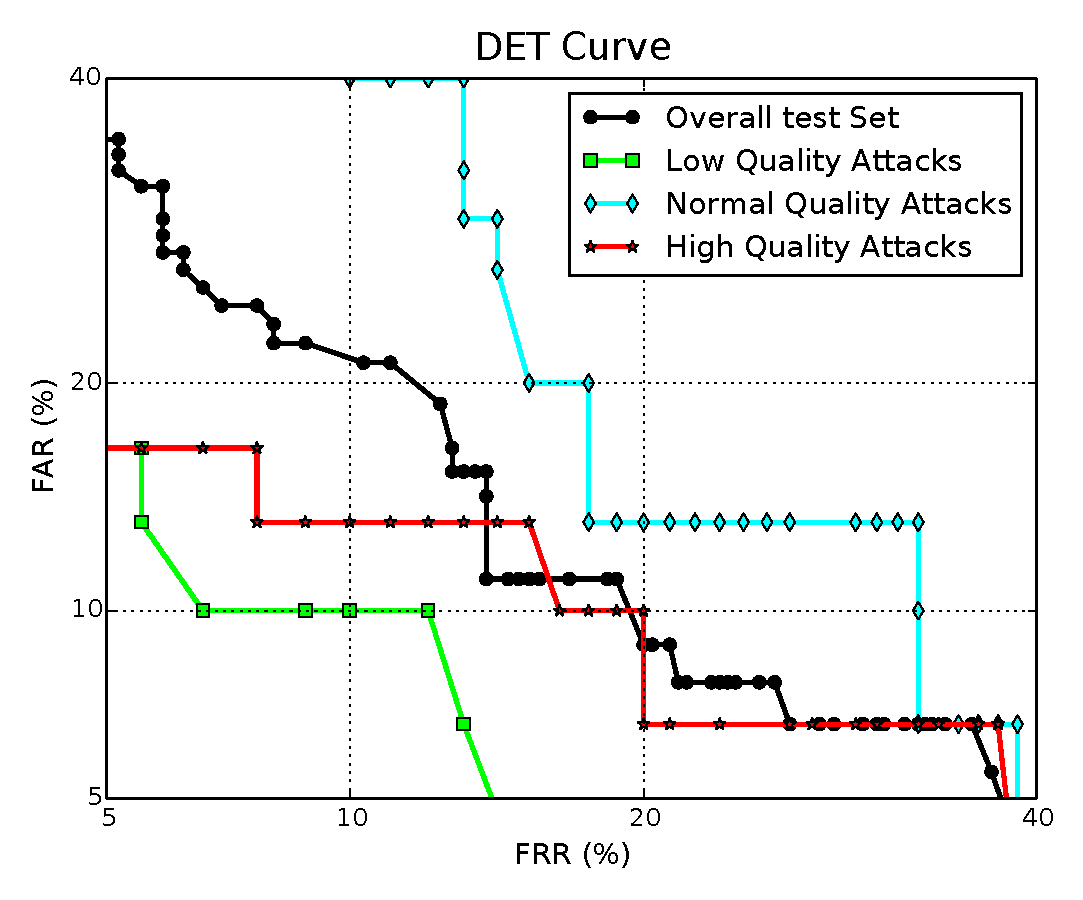
\includegraphics[width=0.45\linewidth]{det_plot_casia_qualy.pdf}}
\caption{Results obtained on CASIA dataset for the three type of attacks (a) and for the three quality of attack (b).}
\label{fig:det_plot_casia}
\end{figure}


\subsubsection{3DMAD Dataset}\label{subsec:3dmad_results}
We now turn our attention \minor{to evaluate} the proposed method for mask-based spoofing attack detection {using the Protocol IV (c.f., Sec.~\ref{subsec:Protocol})}. Using the official \minor{dataset protocol}, the proposed method obtained an AUC of $96.16\%$ and an HTER of $8.0\%$.

\minor{Erdogmus et al.~\cite{Erdogmus:BTAS:2013} reported an HTER of $0.95\%$ using block-based LBP features (local features) and the Linear Discriminant Analysis (LDA) classifier. This performance difference is somewhat explained due to the different validation protocol used. Erdogmus et al. used an $1000$-fold cross validation method and, in each fold, the clients from the dataset were randomly assigned into training, development and test sets. In our case, we randomly divided the clients from dataset and assigned them into training, development and test set only once. Even so, the proposed method outperforms other techniques using global LBP, whose HTERs reported by Erdogmus et al. were all above $10.0\%$.}


\subsubsection{UVAD Dataset}\label{subsec:uvad_results}
In this experiment, we evaluate the proposed method using the Protocol III (c.f., Sec.~\ref{subsec:Protocol}) and UVAD dataset. We also evaluate the proposed method considering LBP-based and motion-based countermeasure methods. 

According to Pereira et al.~\cite{Pereira:ICB:2013}, the correlation method presents an HTER of $11.79\%$ on Replay-Attack. {In turn,} LBP$_{8,1}^{u2}$~\cite{Chingovska:BIOSEG:2012} was effective to characterize the artifacts embedded in the attack videos on Replay-Attack obtaining an HTER of $15.16\%$. In the UVAD dataset, however, both methods obtained a more modest performance as Table~\ref{tab:antispoofing_uvad} shows. With respect to LBP$_{8,1}^{u2}$ method, for instance, the proposed method reduces the classification error in about $36\%$.
%
\begin{table}[!ht]
	\centering
	\caption{Comparison among LBP-based approach~\cite{Chingovska:BIOSEG:2012}, motion-based approach~\cite{Anjos:IJCB:2011} and the proposed method on the UVAD dataset.}
	\label{tab:antispoofing_uvad}
	\begin{tabular}{cccc}
		\topline
		\headcol \textbf{Methods}                         & \textbf{FAR (\%)} & \textbf{FRR (\%)} & \textbf{HTER (\%)} \\ 
		\midline
		Correlation~\cite{Anjos:IJCB:2011}				  & $81.60$ & $14.56$ & $48.06$ \\
		\rowcol LBP$_{8,1}^{u2}$~\cite{Chingovska:BIOSEG:2012}    & $27.41$ & $66.04$ & $46.72$ \\
		\textbf{Proposed Method} & $\mathbf{44.73}$ & $\mathbf{15.00}$ & $\mathbf{29.87}$ \\
		\bottomline		
	\end{tabular}
\end{table}


%Note that our method was trained with the Replay-Attack dataset and tested with 3DMAD dataset, while the method proposed by Erdogmus~\cite{Erdogmus:BTAS:2013} was trained and tested with samples of the same dataset. Even in with the differences existing between the Replay-Attack and 3DMAD dataset (e.g., acquisition sensor, type of attack performed) in this cross-dataset validation protocol, achieved optimal results, which is a remarkable achievement for spoofing detection research.
%%
%\begin{table}[!htb]
%\centering
%%\linethickness{1.5mm}
%\caption{Results (HTER) obtained with our method and with the one proposed method by Erdogmus et al.~\cite{Erdogmus:BTAS:2013} using the 3DMAD dataset.}
%\label{table:3dmad_result}
%\begin{tabular}{lr}
%\toprule
%\multicolumn{1}{c}{Methods} & HTER (\%) \\
%\toprule
% Erdogmus et al.~\cite{Erdogmus:BTAS:2013} & $0.95$ \\
% Proposed Method &  $8.00$ \\
%\bottomrule
%\end{tabular}
%\end{table}

\subsubsection{Comparison with State-of-the-Art Methods for CASIA and Replay-Attack Datasets}

In this section, we compare the proposed method with others \minor{available} in the literature for Replay-Attack and CASIA datasets. Table~\ref{table:CSA} shows results for the Replay-Attack Dataset. The proposed method outperforms the ones based on texture analysis~\cite{Chingovska:BIOSEG:2012,Maatta:IJCB:2011,Pereira:JIVP:2014} and also methods based on motion analysis~\cite{Anjos:IJCB:2011}. It was also more effective than methods based on fusion schemes reported by Pereira et al.~\cite{Pereira:ICB:2013} and Komulainen et al.~\cite{Komulainen:ICB:2013}, with a relative error reduction (RER) of \allan{$67.69\%$ and $46.18\%$}, respectively.
%
\begin{table}[!htb]
\centering
%\linethickness{1.5mm}
\caption{Comparison among the existing methods. The first column shows the HTERs reported by the authors, whereas the second column shows the Relative Error Reduction (RER) obtained with the proposed method. The reported HTERs were obtained using the original Replay-Attack Dataset~\cite{Chingovska:BIOSEG:2012} protocol. \allan{The results highlighted with~$\dagger$~and~$\ddagger$~were reported by Chingovska et al.~\cite{Chingovska:BIOSEG:2012} and Pereira et al.~\cite{Pereira:ICB:2013}, respectively.}}
\label{table:CSA}
\begin{tabular}{lcc}
\topline
\headcol \multicolumn{1}{c}{Methods} & HTER (\%) & RER (\%) \\
\midline
 Chingovska et al.~\cite{Chingovska:BIOSEG:2012} & {15.16} & \allan{81.86} \\
 \rowcol Pinto et al.~\cite{Pinto:TIFS:2015} & 14.27 & \allan{80.73} \\
 \allan{M\"{a}\"{a}tt\"{a} et al.}~\cite{Maatta:IJCB:2011} & 13.87$^\dagger$ & \allan{80.17} \\
 \rowcol \allan{Anjos and Marcel}~\cite{Anjos:IJCB:2011} & 11.79$^{\ddagger}$ & \allan{76.68} \\
 Pereira et al.~\cite{Pereira:ICB:2013} & 8.51 & \allan{67.69} \\
 \rowcol Pereira et al.~\cite{Pereira:JIVP:2014} & 7.60 & \allan{63.82} \\
 Komulainen et al.~\cite{Komulainen:ICB:2013} & 5.11 & \allan{46.18} \\
 \rowcol \textbf{Proposed Method} &  \textbf{2.75} & 0 \\
\bottomlinec
\end{tabular}
\end{table}

Table~\ref{table:soa_casia} shows a comparison among the proposed method and others reported in the literature for CASIA dataset. The proposed method is on par with the best ones in the literature.
%
\begin{table}[!htb]
\centering
%\linethickness{1.5mm}
\caption{Comparison among the proposed method and others available in the literature. According to the authors of the proposed methods, EERs reported were obtained using the original CASIA Dataset~\cite{Zhang:ICB:2012} protocol.}
\label{table:soa_casia}
\begin{tabular}{lr}
\topline
\headcol \multicolumn{1}{c}{Methods} & EER (\%) \\
\midline
 DoG Baseline.~\cite{Zhang:ICB:2012} & 17.0 \\
 \rowcol LBP$_{8,1}^{u2}$.~\cite{Pereira:JIVP:2014} & 16.0 \\
 LBP-TOP$_{8,8,8,1,1,1}^{u2}$.~\cite{Pereira:JIVP:2014} & 10.0 \\
 \rowcol \textbf{Proposed Method}  &  \textbf{14.0} \\
\bottomlinec
\end{tabular}
\end{table}
%
%Finally, Table~\ref{table:CC} shows the results obtained with our method and the teams that participated in the 2013 2nd Competition on Counter Measures to 2D Face Spoofing Attacks~\cite{Chingovska:ICB:2013}. In this comparison, the proposed method is more effective than those methods without fusion schemes and even some using fusion. Note that the choice of parameters for validating our method on CASIA dataset was made using the Replay-Attack dataset. This shows the robustness of our proposed method which were not fully optimized for the dataset in question as many approaches in the literature. We opted for this strategy as we believe it is more realistic in a real-world setting.
%%In this competition, the teams to train ours algorithms using the Replay-Attack and to test them using anonymous test that was built with real samples from Replay-Attack. 
%%
%\begin{table}[!htb]
%\scriptsize
%\centering
%%\linethickness{1.5mm}
%\caption{Results in terms of HTER obtained with our method and with the teams that participated in the 2013 2nd Competition on Counter Measures to 2D Face Spoofing Attacks promoted by the International Conference on Biometrics (ICB)~\cite{Chingovska:ICB:2013}.}
%\label{table:CC}
%\begin{tabular}{lccccccc}
%\topline
%\headcol & \multicolumn{3}{c}{Development} & \multicolumn{3}{c}{Test} & \\
%%\cmidrule(l){2-4}
%%\cmidrule(r){4-7}
%\headcol \multicolumn{-1}{c}{Methods} & FAR & FRR & HTER & FAR & FRR & HTER & Fusion\\
%\midline
%CASIA    & 0.00  & 0.00 & 0.00 & 0.00  & 0.00  & 0.00  & $\checkmark$ \\
%\rowcol IGD      & 5.00  & 8.33 & 6.67 & 17.00 & 1.25  & 9.13  & $\checkmark$ \\
%MaskDown & 1.00  & 0.00 & 0.50 & 0.00  & 5.00  & 2.50  & $\checkmark$ \\
%\rowcol LNMIIT   & 0.00  & 0.00 & 0.00 & 0.00  & 0.00  & 0.00  & $\checkmark$ \\
%MUVIS    & 0.00  & 0.00 & 0.00 & 0.00  & 2.50  & 1.25  & $\checkmark$ \\
%\rowcol PRA Lab  & 0.00  & 0.00 & 0.00 & 0.00  & 2.50  & 1.25  & $\checkmark$ \\
%ATVS     & 1.67  & 0.00 & 0.83 & 2.75  & 21.25 & 12.00 &  \\
%\rowcol Unicamp  & 13.00 & 6.67 & 9.83 & 12.50 & 18.75 & 15.62 &  \\
%\textbf{Proposed Method}  & \textbf{5.00} & \textbf{5.00} & \textbf{5.00} & \textbf{2.00} & \textbf{15.00} & \textbf{8.5} \\
%\bottomline
%\end{tabular}
%\end{table}

%Comparing our method with the ones reported in the literature, our approach presents better results than methods based on texture analysis~\cite{Chingovska:BIOSEG:2012,Maatta:IJCB:2011,Pereira:JIVP:2014} and methods based on motion analysis~\cite{Anjos:IJCB:2011}. Moreover, our approach was more effective than methods based on fusion schemes~\cite{Pereira:ICB:2013,Komulainen:ICB:2013}. {The results shown in Table~\ref{table:CC} reinforce the effectiveness of the proposed method when compared to other solutions without fusion schemes.}

%The CASIA  team proposed a feature-level fusion between one texture descriptor and three motion descriptors. The authors use a multi-scale version of the Linear Binary Patterns (LBP) and  the Gunnar Farneback's algorithm~\cite{Bigun:LNCS:2013} for extracting dense optical flows between two frames of three regions of the scene: head, torso, and background. The team LNMIIT proposed a feature-level fusion for texture and motion-based descriptors. The authors used the LBP to extract micro-texture patterns present in the face region and non-rigid motion analysis approach proposed by Yan et al.~\cite{Yan:ICARCV:2012}.

%Even though there are many studies in the literature showing that the combination of texture and motion-based approaches is a suitable strategy for detecting spoofing attacks~\cite{Yan:ICARCV:2012,Chingovska:ICB:2013,Komulainen:ICB:2013}, we must ensure whether the assumptions made by the motion-based methods (e.g., stationary recognition system, static background) makes sense in a real scenario where the system will be implemented. The assumptions required by the motion-based method are not always satisfied in the scenarios wherein the identifications are made in a totally uncontrolled environment as occur with authentication systems implemented in mobile devices. We do not make such assumptions with the proposed method herein. Finally, any fusion method can also take advantage of our method by adding it to their fusion schemes aiming at improving the final decision of the spoofing attack detection system.

\subsubsection{Analysis of the Minimum Detection Time}\label{subsec:n_frames}

\minor{We now analyze the impact of the video length over the method discriminability for CASIA, Replay-Attack and 3DMAD datasets. This experiment evaluates: the minimum number of frames required for the method to operate; and the method stability, in terms of HTER(\%), for the three different datasets.}

Fig.~\ref{fig:n_frames} indicates that HTER values vary only slightly when we change the video length for the three datasets and that the proposed method uses about two seconds to detect an attempted attack, thus not compromising the transparency of the authentication process.
%
\begin{figure}[h]
\centering
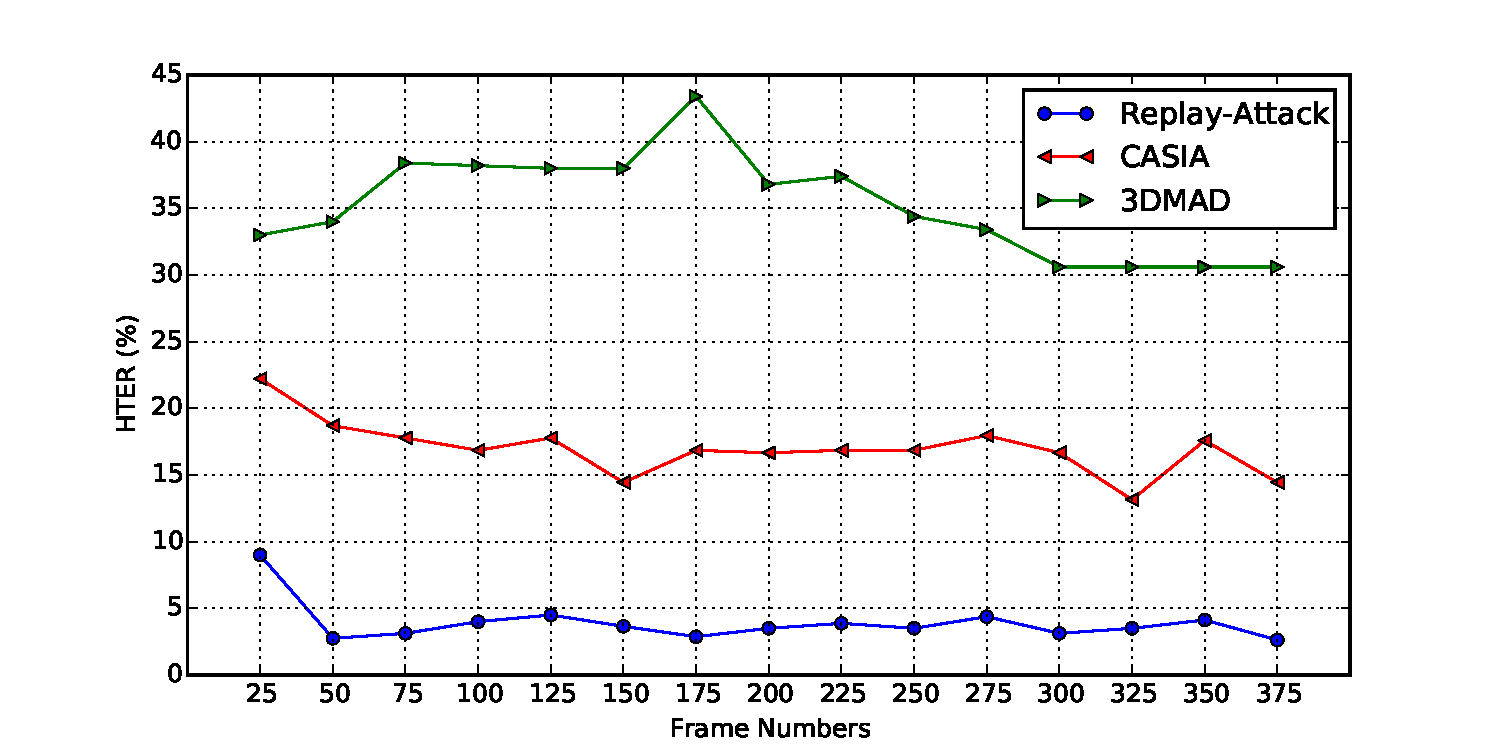
\includegraphics[width=0.45\textwidth]{./figures/n_frames}
\caption{Results in terms of HTER (\%) of the proposed method for different video input length for Replay-Attack, CASIA and 3DMAD datasets.}
\label{fig:n_frames}
\end{figure}

\subsubsection{Cross-Dataset Evaluation}\label{subsec:OtherDatabase}
\minor{In this section, we discuss the performance of the proposed method considering a more difficult scenario (cross-dataset), in which the proposed method is trained with one dataset but it is tested on a different dataset with different acquisition conditions. In this experiment, all datasets used during the training were randomly divided into training and development sets in a proportion of $80\%$ and $20\%$, respectively. The development set is used to estimate the EER threshold that is necessary to calculate the HTER during the test.}

Table~\ref{tab:cross-dataset} shows the results using the cross-dataset protocol. The results indicate that the proposed method presents better generalization when trained with CASIA, with a mean HTER of $40.17\%$. We believe this occurred due to more variability of the type of attacks and video quality in the CASIA dataset, which enriches the training. This dataset contains warped-, cut- and video-based attacks performed with spoofed samples of different quality: low, normal and high quality. Such characteristics enables a better generalization of the method when CASIA is used for training.

{In turn, the best performance when testing the CASIA and 3DMAD datasets was obtained when training with UVAD dataset, another rich dataset for training. Although this dataset contains only video-based spoofing attacks, it has comprises different sensors (for capturing and recapturing the biometric samples) and display devices used during the attempted attacks. We believe that such variability adds different sensor-intrinsic noise levels to the training samples, which contribute to build a more robust classification model.}

{With regard to the more modest generalization presented during the test of the 3DMAD dataset, we believe that it is due to the absence of some artifacts that are commonly found in samples from photo-based and video-based attacks (e.g., blurring, flickering effects) that were not found in the attempted attack video from 3D masks. In addition, spoofing attacks performed with masks are less likely to add temporal disturbances similar to those added when the impostor presents the fake samples, by hand, using a monitor or a photo.}

\minor{Finally, Table~\ref{tab:cross_comparison} shows a comparison among the obtained results reported in the literature. Except for the correlation method, all others present a better performance when they are trained with CASIA. Once again, we believe that our method performs better when training with CASIA because such dataset is more heterogeneous than Replay-Attack. The Correlation~\cite{Anjos:IJCB:2011} and LBP-TOP~\cite{Chingovska:BIOSEG:2012} methods aim to characterize temporal information, similarly to the proposed method, and the results of both methods emphasize the difficulty in characterizing such information completely. In this protocol, besides handling data from different sensors, all methods have to deal with different lighting conditions and background.}

%
%%
%\begin{table}[!htb]
%\scriptsize
%\centering
%%\linethickness{1.5mm}
%\caption{Results in terms of HTER obtained with our method using the cross-dataset Protocol.}
%\label{table:cross}
%\begin{tabular}{lccc}
%\toprule
%\textbf{Datasets} & FAR & FRR & HTER \\
%\toprule
%CASIA  & 11.11 & 83.33 & 47.22 \\
%3DMAD  & 29.41 & 52.94 & 41.18 \\
%UVAD   & 1.34  & {87.17} & {44.26} \\
%\bottomrule
%\end{tabular}
%\end{table}
%
\begin{table*}[!ht]
	\centering
	\footnotesize
	\caption{Results obtained with the cross-dataset protocol and using the overall test sets of each dataset.}
	\label{tab:cross-dataset}	
	\begin{tabular}{cccccc}
		\topline
		\headcol \textbf{Train} & \textbf{Test} & \textbf{FAR (\%)} & \textbf{FRR (\%)} & \textbf{HTER (\%)} & \textbf{Mean HTER (\%)} \\  
		\midline
		%
		& 3DMAD         & 88.00 & 4.00  & 46.00 & \\
		\rowcol 						& Replay-Attack & 32.50 & 36.25 & \textbf{34.38} & \\
		\multirow{-3}{*}{CASIA}         & UVAD          & 38.61 & 41.67 & \textbf{40.14} & \multirow{-3}{*}{ $40.17\%$ } \\
		%
		\hline
		\rowcol									& 3DMAD & 52.00 & 44.00 & 48.00 & \\
		\rowcol									& CASIA & 0.00 & 100.0 & 50.00 & \\
		\rowcol \multirow{-3}{*}{Replay-Attack} & UVAD  & 5.74 & 83.33  & 44.54 & \multirow{-3}{*}{ $47.45\%$ } \\
		%
		\hline
		& 3DMAD         & 84.00 & 4.00  & \textbf{44.00} & \\
		\rowcol							& CASIA         & 13.70 & 63.33 & \textbf{38.52} & \\										
		\multirow{-3}{*}{UVAD}          & Replay-Attack & 79.25 & 6.25 & 42.75  & \multirow{-3}{*}{ $41.76\%$ } \\
		\bottomline 
	\end{tabular} 
\end{table*}
%

%The results show that our method is still not the final word considering a cross-dataset validation (training with one dataset and testing in a different dataset). However, according to other results reported in the literature recently, this behavior is expected, as reported by Pereira et al.~\cite{Pereira:ICB:2013}, whose results in Table~\ref{table:cross_compar} corroborate our findings. We believe that this difficulty of the methods in classifying data from other datasets, not seen during training, is partly because of the different conditions for the acquisition of real samples and recapture of false samples. Therefore, we recommend that either our method is optimized according to the target operational setup or that the method is trained using a good representation of the operational setup of the testing, in other words, the training must comprise examples of situations that could appear during testing. The more complex is the training set the more likely the method will generalize.

%Finally, note that we are not proposing the final word on cross-dataset evaluation. This is a much more challenging problem and here we only touch the tip of the iceberg. Much more work still needs to be done in this direction from all of the research community.
%
%\begin{table}[!htb]
%\scriptsize
%\centering
%%\linethickness{1.5mm}
%\caption{Cross-dataset evaluation comparison of the proposed method with the ones reported in~\cite{Pereira:ICB:2013} for CASIA dataset.}
%\label{table:cross_compar}
%\begin{tabular}{lr}
%\toprule
%\textbf{Datasets} & HTER (\%) \\
%\toprule
%Our method              	 & 47.22   \\
% \hline
%Correlation Motion           & 48.28 \\
%$LBP_{8,1}^{u2}$             & 57.90  \\
%$LBP-TOP_{8,8,8,1,1,1}^{u2}$  & 61.33 \\
%\bottomrule
%\end{tabular}
%\end{table}

%UVAD dataset which contains attempted attacks performed with high quality devices. With this experimental protocol, we obtain an AUC of $94.86\%$ and a HTER of $12.50\%$, considering all attempted attack videos contained on the UVAD dataset. Fig.~\ref{fig:uvad_barplots} shows the results for each sensor acquisition and display devices in the UVAD dataset. The proposed method was capable of capturing noise and artifacts added in the synthetic biometric samples even when the attempted attacks are performed with high quality videos, for different display devices used in the attacks and different biometric sensors. We can conclude that the assumptions made in this work, regarding the perturbations in the frequency components of the signal captured by the acquisition sensor caused by adding noise and artifacts are consistent and generalizable to other attack scenarios.
%%
%\begin{figure*}[!htb]
%\centering
%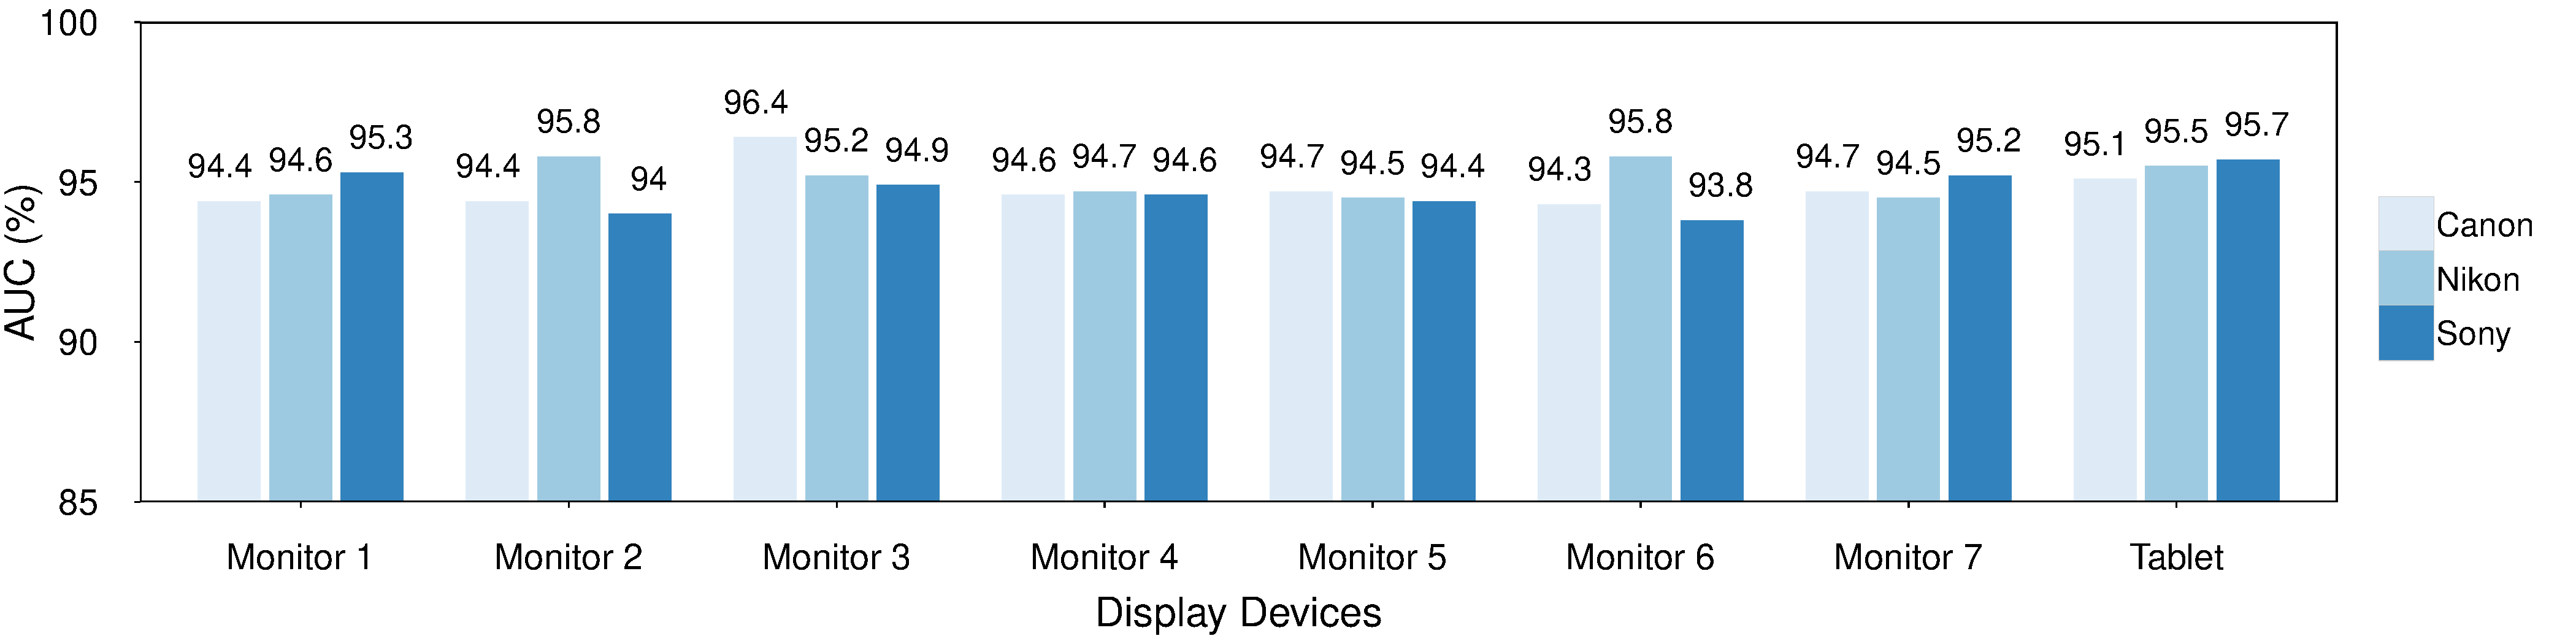
\includegraphics[width=0.99\textwidth]{UVAD_Barplot.pdf}
%\caption{Results (AUC) of the cross-dataset experiment analyzing the different attacks presents on the UVAD dataset. The attacks were performed in three sensor acquisition using eight different display devices.%\newtodo{Remover o fundo cinza.}
%}
%\label{fig:uvad_barplots}
%\end{figure*}
